%=====================================================================
% EBSSC_full.tex
% Entropy-Bounded Sparse Semantic Calculus (EBSSC)
% Full draft: Sections 1-18 + Appendices A-F
% Author: Flyxion
%=====================================================================
\documentclass[11pt,a4paper]{article}
\usepackage[margin=1in]{geometry}
\usepackage{amsmath,amssymb,amsthm,amsfonts}
\usepackage{hyperref}
\usepackage{graphicx}
\usepackage{listings}
\usepackage{xcolor}
\usepackage{bm}
\usepackage{mathrsfs}
\usepackage{microtype}
\usepackage{tikz}
\usepackage{enumitem}
\usepackage{booktabs}
\usepackage{float}
\usepackage{longtable}
\usepackage{caption}
\usepackage{array}
\usepackage{multirow}
\usepackage{natbib}

\title{\textbf{Entropy-Bounded Sparse Semantic Calculus (EBSSC)}\\
A Unified Syntax and Semantics for SpherePOP and Latent Policy Selection}
\author{Flyxion\\ \small{\textit{A Relativistic Scalar–Vector Plenum (RSVP) Project}}}
\date{\today}

\newtheorem{theorem}{Theorem}[section]
\newtheorem{definition}{Definition}[section]
\newtheorem{proposition}{Proposition}[section]
\newtheorem{lemma}{Lemma}[section]
\newtheorem{corollary}{Corollary}[section]

\newcommand{\E}{\mathbb{E}}
\newcommand{\R}{\mathbb{R}}
\newcommand{\norm}[1]{\left\lVert #1 \right\rVert}

\begin{document}
\maketitle

\begin{abstract}
The \emph{Entropy-Bounded Sparse Semantic Calculus (EBSSC)} provides a unified formalism for integrating the geometric semantics of \textbf{SpherePOP} with the probabilistic control structure of \textbf{Latent Policy Selection}. EBSSC treats thought, inference, and concept formation as policy-driven evolutions on fields of meaning (semantic spheres) constrained by entropy and sparsity budgets. We define the formal syntax, typing, and operational semantics; prove entropy soundness and stability; present a sparse free-energy objective; and show an explicit isomorphism between EBSSC dynamics and unistochastic transition operators. The result is a compositional calculus where semantic coherence, cognitive economy, and physical information constraints coincide under a single variational principle.
\end{abstract}

\tableofcontents
\clearpage

%=====================================================================
\section{Introduction}
%=====================================================================


\section{Introduction}

Cognition, collaboration, and concept formation can be understood as constrained processes operating over structured internal representations.
The \emph{free-energy principle} frames biological agents as systems that minimize a variational bound on surprise \cite{friston2006free,friston2010free}, an approach generalized in active inference to include planning and epistemic action \cite{friston2019active,parr2022markov}.
Separately, sparse coding and compressed sensing demonstrate that high-dimensional signals can be reconstructed from a small number of active components if the basis and sparsity structure are appropriate \cite{tibshirani1996lasso,donoho2006compressed,donoho2009observed}.

However, cognitive theories emphasizing inference rarely formalize the \emph{structure of meaning itself}, while semantic knowledge systems lack a principled theory of action selection or uncertainty minimization.
This paper presents the \emph{Entropy-Bounded Sparse Semantic Calculus (EBSSC)}, a computational and mathematical framework that unifies:

\begin{enumerate}
    \item \textbf{Structured semantic representations}, modeled as \emph{semantic spheres}, drawing inspiration from information geometry \cite{amari2016information,baez2011information}, semantic energy formulations \cite{feygin2020meaning}, and category-theoretic process models \cite{coecke2017picturing,baez2017entropy};
    \item \textbf{Goal-directed cognition as policy selection}, expressed as sparse variational inference over latent action spaces \cite{friston2010free,friston2019active,rezende2014stochastic};
    \item \textbf{Entropy-constrained semantic evolution}, in which concept dynamics obey bounded information growth, analogous to entropy production constraints in thermodynamic and open systems \cite{jaynes1957information,finn1982entropy,van2010three}.
\end{enumerate}

EBSSC models a cognitive or communicative act as a \emph{policy-induced transformation of a semantic field}, constrained by:

(i) bounded semantic entropy, preventing representational drift,

(ii) sparse policy activation, enforcing computational and cognitive parsimony, and

(iii) type-governed compositionality, ensuring semantic well-formedness.

This results in a calculus which is simultaneously:

\begin{itemize}
    \item \emph{variational}, minimizing a free-energy objective \cite{friston2006free,caticha2015entropic};
    \item \emph{sparse}, selecting minimal policy support \cite{tibshirani1996lasso,donoho2006compressed};
    \item \emph{semantic}, maintaining structured concept geometry \cite{amari2016information,feygin2020meaning};
    \item \emph{categorical}, forming a bounded monoidal category of semantic morphisms \cite{maclane1971categories,lurie2009higher,baez2011physics};
    \item \emph{information-theoretic}, admitting unistochastic transition semantics \cite{barandes2022unistochastic}.
\end{itemize}

\subsection{Motivating Gap}

Three limitations motivate the construction of EBSSC:

\textbf{1. Free-energy models lack semantic state structure.}  
Active inference models treat hidden states as latent variables but do not specify the geometry or compositional structure of \emph{meaning itself} \cite{friston2010free,parr2022markov}.

\textbf{2. Semantic representations lack cognitive selection principles.}  
Semantic network models and embedding spaces do not inherently explain \emph{why} particular conceptual updates occur rather than others.

\textbf{3. Neither framework bounds semantic drift.}  
Without explicit entropy budgets, iterative updates can accumulate unbounded noise or inconsistency, violating long-term conceptual coherence \cite{baez2017entropy,jaynes1957information}.

---

\subsection{Contributions}

This paper contributes:

\begin{enumerate}
    \item A typed operational calculus for semantic state transitions (\S3) grounded in small-step semantics.
    \item A variational objective combining free-energy, sparsity, and policy cost (\S4), whose solutions obey LASSO-style phase transitions \cite{tibshirani1996lasso,donoho2009observed}.
    \item Formal guarantees of \textbf{progress}, \textbf{preservation}, and \textbf{entropy budget safety} (\S5), ensuring well-typed updates remain semantically bounded.
    \item A categorical formulation of semantic compositionality as a symmetric monoidal closed structure (\S6) \cite{maclane1971categories,coecke2017picturing}.
    \item A constructive mapping to unistochastic quantum-like transition dynamics (\S7) \cite{barandes2022unistochastic,mackey1963mathematical}.
\end{enumerate}

---

\subsection{Notational conventions}

\begin{center}
\begin{tabular}{ll}
$\sigma$ & Semantic sphere (a structured concept representation) \\
$\pi$ & Policy acting on semantic fields \\
$E(\sigma)$ & Semantic entropy \\
$G(\sigma,\pi)$ & Expected free energy of executing $\pi$ on $\sigma$ \\
$\Lambda$ & Sparsity pressure coefficient ($\ell_1$ penalty) \\
$C(\pi)$ & Policy execution cost \\
$\Gamma$ & Global semantic context (plenum) \\
$\oplus,\;\ominus,\;\circledast$ & Pop, collapse, and merge operators
\end{tabular}
\end{center}

In the \emph{SpherePOP} framework, concepts and percepts are represented as structured manifolds—semantic spheres—whose internal geometry encodes coherence and boundary structure. In the \emph{Latent Policy Selection} model, cognition is described as sparse Bayesian control in a latent plenum: an agent selects a minimal-complexity policy that minimizes expected free energy.

EBSSC fuses these views into a single semantic-operational calculus. Each act of thought becomes a policy application to a semantic sphere, constrained by entropy budgets and sparsity penalties. The calculus therefore unifies symbolic, geometric, and variational formulations of meaning.

\subsection{Overview}
EBSSC is defined by:
\begin{enumerate}[label=\textbf{\arabic*.}]
\item A \textbf{typed syntax} of sphere-level operations (pop, merge, collapse, rewrite, etc.).
\item An \textbf{operational semantics} describing entropy-bounded transitions.
\item A \textbf{sparse free-energy objective}
  \[
  \pi^*=\arg\min_\pi \big[G(\sigma,\pi)+\Lambda\norm{\pi}_1+\gamma C(\pi)\big],
  \]
  balancing expected free energy, sparsity, and cost.
\item \textbf{Soundness theorems} ensuring entropy and sparsity stability.
\item A \textbf{categorical interpretation} as a monoidal category of bounded morphisms.
\end{enumerate}


%=====================================================================
\section{Geometry of Semantic Spheres and Fields}
%=====================================================================

This section leads with geometry: manifolds, fields, and how semantic spheres arise as bounded regions with boundary structure and internal fields encoding meaning.

\subsection{Manifolds to Fields}
Let \(M\) be a smooth manifold representing the semantic plenum. A semantic field is a scalar or vector-valued function \(\Phi: M \to \R^k\) that encodes distributed semantic activation. Regularity conditions (smoothness, finite energy) are imposed so that \(\Phi\) admits meaningful gradients and a well-defined boundary flux.

\subsection{Spheres and Boundaries}
A semantic sphere \(\sigma\) is a compact region \(B \subset M\) together with its boundary \(\partial B\). The internal field \(\Phi|_B\) and boundary conditions on \(\partial B\) determine local coherence. The boundary operator \(\partial\) encodes interfaces for merge and transport operations.

\subsection{Field Geometry and Semantic Metrics}
Equip \(M\) with an information metric derived from Fisher information on distributions induced by \(\Phi\). Curvature notions are used to define semantic sharpness and concept locality: low curvature regions correspond to well-formed concepts.

%=====================================================================
\section{Syntax: Spheres, Policies, and Programs}
%=====================================================================

\subsection{Core symbols and intuition}
\begin{center}
\begin{tabular}{ll}
$\sigma$ & Semantic sphere (conceptual unit)\\
$\pi$ & Policy operator acting on spheres\\
$\Gamma$ & Global semantic plenum (context)\\
$E(\sigma)$ & Semantic entropy\\
$C(\pi)$ & Policy cost\\
$G(\sigma,\pi)$ & Expected free energy\\
$\Lambda$ & Sparsity pressure (L1 constraint)\\
$\oplus,\ \ominus,\ \circledast$ & Pop / collapse / merge\\
$\partial$ & Boundary operator\\
$\langle\ \rangle$ & Provenance trace
\end{tabular}
\end{center}

\subsection{Sphere structure}
\[
\sigma := \{\Phi,\partial\Phi,M,H,T\}
\]
where \(\Phi\) is an internal semantic field, \(\partial\Phi\) its boundary, \(M\) a memory trace, \(H\) an entropy history, and \(T\) a type signature describing admissible operations.

\subsection{Policy grammar (summary)}
\begin{align*}
\pi ::= {}& \mathrm{pop}(\sigma)
 \mid \mathrm{merge}(\sigma_1,\sigma_2)
 \mid \mathrm{collapse}(\sigma)
 \mid \mathrm{bind}(\sigma_1\!\to\!\sigma_2) \\
 &\mid \mathrm{rewrite}(\sigma,r)
 \mid \mathrm{mask}(\sigma,m)
 \mid \mathrm{allocate}(\sigma,b).
\end{align*}

\subsection{Well-formed programs}
A program is a trace of sphere transitions
\[
P := \langle\sigma_0\rangle \xrightarrow{\pi_1} \langle\sigma_1\rangle \xrightarrow{\pi_2} \cdots \xrightarrow{\pi_k} \langle\sigma_k\rangle
\]
subject to
\[
\norm{P}_0\le\Lambda,\qquad
\sum_i C(\pi_i)\le B,\qquad
T(\sigma_i)\models \pi_i.
\]

%=====================================================================
\section{Operational Semantics and Small-Step Rules}
%=====================================================================

\subsection{Small-step semantics}
We adopt a small-step judgement of the form:
\[
(\sigma,\Gamma)\xrightarrow{\pi}(\sigma',\Gamma')
\]
and program-level reduction:
\[
\frac{(\sigma,\Gamma)\xrightarrow{\pi}(\sigma',\Gamma')}{\langle\sigma\rangle :: P \to \langle\sigma'\rangle :: P'}.
\]

\subsection{Core transition rules}

\paragraph{Pop (expansion).}
\[
\sigma\oplus \xrightarrow{\pi} \sigma' \quad\text{iff}\quad
E(\sigma')\le E(\sigma)+\varepsilon,\quad C(\pi)\text{ minimal.}
\]

\paragraph{Merge (fusion).}
\[
\sigma_1\circledast\sigma_2\xrightarrow{\pi}\sigma_3
\quad\text{iff}\quad
\begin{cases}
\text{boundary\_compatible}(\sigma_1,\sigma_2),\\
G(\sigma_3,\pi)<G(\sigma_1,\pi)+G(\sigma_2,\pi),\\
E(\sigma_3)\le E(\sigma_1)+E(\sigma_2)-\delta.
\end{cases}
\]

\paragraph{Collapse (pruning).}
\[
\sigma\ominus\xrightarrow{\pi}\sigma' \quad\text{iff}\quad
I(\sigma')\ge I_{\min},\ 
E(\sigma')<E(\sigma),\
C(\pi)<G(\sigma,\pi).
\]

\subsection{Typing judgments and safety}
We write typing judgments \(\Gamma \vdash \pi : \sigma \Rightarrow \sigma'\) to assert admissibility and entropy-budget compliance of policy actions. Progress and preservation theorems are proved in Appendix B.

%=====================================================================
\section{Entropy-Bounded Optimization}
%=====================================================================

The fundamental objective combines Fristonian free energy with L1 sparsity:
\[
\pi^* = \arg\min_\pi \big[G(\sigma,\pi)+\Lambda\norm{\pi}_1+\gamma C(\pi)\big].
\]
$G$ encodes both extrinsic surprise and intrinsic complexity. Sparsity pressure $\Lambda\norm{\pi}_1$ enforces minimal active policies; $\gamma C(\pi)$ measures metabolic or computational cost.

We analyze existence (Weierstrass), KKT conditions, and phase transitions in Appendix A.

%=====================================================================
\section{SpherePOP Operators and Extensions}
%=====================================================================

SpherePOP provides operational primitives used inside EBSSC:

\begin{itemize}
    \item \textbf{pop} — typed expansion/transduction from one modality to another with entropy accounting.
    \item \textbf{merge} — boundary-aware fusion with coherence check and entropy decrease criterion.
    \item \textbf{close} — media-quine closure ensuring declared modalities are populated via rule application.
    \item \textbf{collapse} — pruning operator that consolidates redundant or low-information regions.
    \item \textbf{bind} — causal binding operator that composes policies into higher-order actions.
\end{itemize}

Operational semantics for each operator appear in Section 4 and Appendix C.

%=====================================================================
\section{Typing, Safety, and Meta-Theory}
%=====================================================================

\subsection{Sphere types}
\begin{definition}[Sphere type]
A sphere has signature
\[
\sigma : (T_{\mathrm{in}}\to T_{\mathrm{out}})[E\le\beta,D\le\delta,\deg\le k],
\]
restricting admissible transitions by entropy, depth, and degree.
\end{definition}

\subsection{Main meta-theorems (statements)}
Progress, Preservation, and Entropy Budget Safety are formalized and proved (sketches and full arguments) in Appendix B.

%=====================================================================
\section{Soundness and Stability}
%=====================================================================

\begin{theorem}[Entropy Soundness]
Let $\sigma_0$ be initial, and $\pi_1,\ldots,\pi_n$ be a policy trace satisfying local budgets $\Delta E(\pi_i)\le b_i$. Then
\[
E(\sigma_n)\le E(\sigma_0)+\sum_{i=1}^n b_i.
\]
\end{theorem}

\begin{proof}[Sketch]
Each rule consumes a declared budget $b_i$, bounding $\Delta E_i$. By induction on trace length, the total entropy increase is the sum of per-step budgets. If $\sum b_i\le B$ (global constraint), total entropy is bounded by $E(\sigma_0)+B$. A transition requiring $\Delta E>B$ is ill-typed and cannot execute.
\end{proof}

\begin{proposition}[Stability under sparsity]
If activations $a$ satisfy $\norm{a}_1\le A_{\max}$ and $\Delta E\le\kappa\norm{a}_1$, then global entropy obeys
$E(\sigma_t)\le E_0+\kappa A_{\max}$; the system is Lyapunov-stable.
\end{proposition}

%=====================================================================
\section{Categorical Semantics}
%=====================================================================

EBSSC forms a bounded monoidal category:
\[
\mathcal{C}_{\text{EBSSC}}=(\text{Obj}=\text{Spheres},\ 
\text{Mor}=\text{Policies},\ 
\otimes=\text{Merge}).
\]
Morphisms are entropy-non-increasing, and composition obeys
\[
E(f\circ g)\le E(f)+E(g).
\]

The free-energy functional provides a functor
\[
\mathcal{F}:\mathcal{C}_{\text{EBSSC}}\to (\R_{\ge0},+)
\]
mapping morphisms to expected free energy; monoidal and closed structure and internal Homs correspond to binding and causal composition (see Appendix D for diagrams).

%=====================================================================
\section{Higher Topos and Sheaf Semantics}
%=====================================================================

Semantic sheaves model local-to-global inference: spheres correspond to sections, merge/glue = descent data, and provenance is realized by functorial restriction maps. The sheaf semantics clarifies when and how local inferences compose into global coherent knowledge and formalizes the Media-Quine closure via sheaf-theoretic completeness conditions (definition in Appendix A).

%=====================================================================
\section{Compiler Pipeline and Intermediate Representation}
%=====================================================================

The compiler stack (Section 16 elaborates) maps SpherePOP programs to entropy-safe executable traces:

\begin{enumerate}
    \item Parser $\to$ typed AST.
    \item Type/Budget checker.
    \item Policy optimizer (sparse solver).
    \item Unistochastic lift and execution scheduler.
    \item Runtime enforcing entropy invariants and provenance.
\end{enumerate}

Appendix E contains a formal grammar for the IR, typing rules, and compilation judgments.

%=====================================================================
\section{Unistochastic Correspondence and Quantum Lifts}
%=====================================================================

Following Barandes, discretize \(\Phi\) on \(n\) points, atoms \(\psi_k\) as basis vectors. Extend \(\Psi=[\psi_1,\ldots,\psi_m]\) to a unitary \(U\in\mathbb{C}^{n\times n}\), and define \(B_{ij}=|U_{ij}|^2\). Then \(B\) is unistochastic and describes probabilistic redistribution of semantic mass:
\[
p' = Bp,\qquad p_i=|\Phi_i|^2.
\]
Sparse activation selects columns of \(U\), so EBSSC transitions correspond to column-restricted unistochastic flows (Appendix A contains constructive proofs).

% ============================================================
% SECTION 2 — Manifolding the Latent Plenum: Boundaries, Fields, and Inference Geometry
% ============================================================

\section{Manifolding the Latent Plenum: Boundaries, Fields, and Inference Geometry}

\subsection{Latent Structure as Differentiable Manifold}
Cognitive and decision-theoretic state spaces can be formalized as differentiable manifolds 
endowed with information metrics \cite{amari2016, amari2000}. Learned representations implicitly construct 
coordinate charts over latent state-space \cite{bengio2013}, while generative world models learn transition-smooth 
manifolds of environmental dynamics \cite{hafner2020}. Control systems operating over such spaces must respect 
the induced geometry of constraint manifolds \cite{todorov2009}, and neural population codes exhibit manifold 
alignment properties that govern generalization and transfer \cite{cohen2016}.

\subsection{Field-Theoretic Perspective on Inference and Policy}
Dynamics on latent state spaces can be expressed as fields: scalar potentials, vector flows, 
and entropy-producing channels. Neural computation has been modeled as vector fields governing 
continuous-time dynamics \cite{sussillo2009}. Inference in the variational sense follows gradient descent 
on energy functionals equivalent to free energy \cite{friston2010}, and stochastic inference is driven 
by entropic gradients understood as thermodynamic currents \cite{seifert2012}. Continuous policy 
parameterizations may be formulated as neural ODEs \cite{dupont2019}, whose qualitative behavior 
is constrained by topological invariants \cite{milnor1958}.

\subsection{Compact Latent Domains and Spherical Boundaries}
Bounded latent spaces permit compactification into manifolds with spherical boundary topologies 
\cite{guillemin1974}. Stereographic compactification provides a constructive mapping from 
$\mathbb{R}^n$ to $S^n$ \cite{lee2013}, and sphere-constrained embeddings optimize geodesic efficiency 
under convexity constraints \cite{berger2003}. Spherical harmonics form an orthogonal basis for function 
approximation on compact boundary domains \cite{courant1953}. When inference is cast as entropy minimization 
under compact support, attractor minima localize to the domain boundary \cite{tishby2017}. Boundary conditions 
control global solution structure for field equations posed on such manifolds \cite{evans2022}.

\subsection{Inference Trajectories as Geodesics in Information Space}
Optimal inference and policy traces correspond to geodesics in statistical manifolds equipped 
with the Fisher metric \cite{kakade2002, amari1998}. Path-integral control reveals that energetically 
optimal policies coincide with entropy-weighted geodesics \cite{kappen2012}. In bounded domains, 
stochastic optimal control converges to minimal-action paths terminating at boundary attractors 
\cite{todorov2009}.

\subsection{Spherical Structure in High-Dimensional Decision Boundaries}
Empirical studies show that decision surfaces in deep networks exhibit locally spherical curvature 
properties \cite{fawzi2018}. Hyperspherical embeddings act as stable fixed points for categorical 
partitioning \cite{liu2017}, and normalization onto hyperspherical codes improves separability 
under sparsity pressures \cite{wang2018}.

\subsection{Spherical Packing and the Emergence of Sparse Structure}
Sparsity emerges naturally under spherical packing constraints \cite{donoho2005}. Optimal codes on 
spherical domains minimize expected divergence under information constraints \cite{olshausen1996}. 
Biological systems operating under metabolic limits converge to sparse spherical activation geometries 
due to energy-optimal packing pressures \cite{attwell2001}.

\subsection{Convergence Guarantees Under Compactness}
Compact state domains endow inference maps with fixed-point guarantees \cite{brouwer1911}. If the 
policy update operator is a contraction in a bounded metric space, the optimal policy is unique 
and reachable \cite{bertsekas2017, banach1922}.

% ============================================================
% SECTION 3 — Plenum Fields, Entropy Dynamics, and Latent Policy Flows
% ============================================================

\section{Plenum Fields, Entropy Dynamics, and Latent Policy Flows}

\subsection{Scalar, Vector, and Entropic Components of the Plenum}
We model latent cognition and decision space as a triplet of interacting fields:
\[
\mathcal{P} = (\Phi, \mathbf{v}, S)
\]
where:
\begin{itemize}
    \item $\Phi : \mathcal{M} \to \mathbb{R}$ is a scalar potential encoding pragmatic affordance or expected utility density,
    \item $\mathbf{v} : \mathcal{M} \to T\mathcal{M}$ is a vector field expressing directed policy flux or agentic flow,
    \item $S : \mathcal{M} \to \mathbb{R}_{\geq 0}$ is the entropy field governing informational dispersion.
\end{itemize}
Field-theoretic descriptions of cognition and control have been previously formalized in neural dynamics 
\cite{sussillo2009}, thermodynamic inference \cite{friston2010}, and computational field models of semantics 
\cite{feygin2020}.

\subsection{Entropy as Both Constraint and Curvature}
Following the maximum entropy principle \cite{jaynes1957information}, the entropy field $S$ plays a dual role:
as a regularizer enforcing parsimonious inference and as an information-geometric curvature term shaping the manifold itself \cite{amari2016information}.
On compact domains, high-entropy gradients induce geodesic focusing and boundary attractors \cite{tishby2017}.
The balance between dispersion and compression resembles relative entropy minimization in categorical probability
\cite{baez2017entropy}.

\subsection{Free Energy as the Plenum Action Functional}
Inference trajectories minimize the free energy functional
\[
\mathcal{F}[\pi] = \mathbb{E}_{q_\pi} \left[ -\ln p(o,s) + \ln q_\pi(s) \right],
\]
as in the variational free energy principle \cite{friston2006free, friston2010free}.
Policy selection can be seen as minimizing expected free energy:
\[
\pi^* = \arg\min_\pi \mathbb{E} [G(\pi)],
\]
where $G(\pi)$ combines epistemic and pragmatic value \cite{friston2019active, parr2022markov}.
This action functional can be interpreted as a plenum-wide variational constraint shaping $\Phi$, $\mathbf{v}$, and $S$ simultaneously.

\subsection{Vector Flow as Policy Flux}
The vector field $\mathbf{v}$ is governed by a continuity equation expressing conservation of policy mass:
\[
\frac{\partial \rho}{\partial t} + \nabla \cdot (\rho \mathbf{v}) = \Sigma,
\]
where $\rho$ is policy density and $\Sigma$ is entropy production.\ 
Stochastic thermodynamic interpretations of such flows have been formalized in \cite{seifert2012}.
The field tends toward minimum dissipation paths under constraint, equivalent to path-integral control optima 
\cite{kappen2012}.

\subsection{Entropy Production as a Selection Pressure}
We define entropy production as:
\[
\dot{\Sigma} = \int_{\mathcal{M}} \left( \mathbf{v} \cdot \nabla S + \|\nabla \Phi\|^2 \right) \, d\mu.
\]
Policy flows that increase $\dot{\Sigma}$ are suppressed by sparsity pressure (next section), creating a natural selection landscape over latent actions.
This mirrors dissipative system constraints in physics \cite{finn1982entropy} and bounded rational optimization 
\cite{todorov2009}.

\subsection{Policy Equilibria as Fixed Points of the Plenum Flow}
A stable policy configuration satisfies:
\[
\nabla \cdot (\rho \mathbf{v}) = 0, \quad \nabla \Phi = -\lambda \nabla S,
\]
which corresponds to a generalized thermodynamic equilibrium balancing attractor pull ($\Phi$) against entropic pressure ($S$).
Fixed point existence is guaranteed under compactness by the Brouwer fixed point theorem \cite{brouwer1911},
and uniqueness within a contractive patch by Banach’s fixed point theorem \cite{banach1922}.

\subsection{Emergence of Decision Attractors}
Attractors form where:
\[
\nabla \Phi = 0 \quad \text{and} \quad \nabla S \approx 0,
\]
meaning neither utility gradients nor entropic diffusion dominate.
These correspond to the “crystallized policies” of sparse semantic inference, analogous to representation collapse in neural manifolds \cite{cohen2016} or codebook stabilization in vector quantization \cite{van2017vqvae}.

% ============================================================
% SECTION 4 — Sparse Policy Selection and Compressed Latent Action Spaces
% ============================================================

\section{Sparse Policy Selection and Compressed Latent Action Spaces}

\subsection{Sparsity as Structural, Not Auxiliary}
In classical optimization, sparsity is imposed via an explicit penalty.
In latent policy spaces, sparsity emerges structurally from three independent pressures:

\begin{itemize}
    \item Energetic cost of policy activation (biophysical or computational)
    \item Entropy suppression under inference pressure
    \item Geometric compression of decision manifolds
\end{itemize}

This echoes natural sparsity in neural codes \cite{tibshirani1996lasso}, 
compressed sensing phase transitions \cite{donoho2006compressed}, 
and sparse attractor dynamics in neural manifolds \cite{cohen2016}.

Thus, the plenum does not apply sparsity --- it is sparse by default.


\subsection{Sparse Policy Optimization}
A policy $\pi$ is represented as a latent action vector $a \in \mathbb{R}^n$ with objective:
\[
\min_{a} \Big( \mathcal{L}(a) + \lambda \|a\|_1 + \gamma C(a) \Big)
\]
where:

- $\mathcal{L}(a)$ is task-relevant loss or expected free energy,
- $\lambda \|a\|_1$ enforces sparsity in activated policies,
- $C(a)$ is an entropy-budget constraint inherited from the plenum:
  \[
  C(a) = \int |\nabla S \cdot a(x)| \, dx.
  \]

This connects directly to the LASSO formulation \cite{tibshirani1996lasso} and convex optimization under energy budgets \cite{boyd2004convex}.

\subsection{Phase Transition in Policy Complexity}
Sparse policy spaces exhibit a sharp critical threshold in $\lambda$ where the number of active policies collapses discontinuously:

\[
\lambda_c \approx \sqrt{2 \log n} \ \frac{\sigma}{\|X^\top X\|},
\]

analogous to the Donoho–Tanner phase boundary for high-dimensional recovery \cite{donoho2009observed}.

For $\lambda > \lambda_c$:
- Policy activations collapse to minimal stable attractors.
- Decision variance sharply decreases.
- Exploration capacity vanishes.

For $\lambda < \lambda_c$:
- Policy populations expand explosively.
- Entropy exceeds budget feasibility.
- Decision flows destabilize.

This defines a *navigability corridor* in latent space where sparse agency exists without collapse.

\subsection{Policy Pruning as Proximal Flow}
Evolution of policy weights proceeds via proximal descent:
\[
a_{k+1} = \operatorname{prox}_{\lambda \|\cdot\|_1}(a_k - \eta \nabla \mathcal{L}(a_k)),
\]
using the proximal operator \cite{moreau1965proximite}:

\[
\operatorname{prox}_{\lambda\|\cdot\|_1}(x) = \mathrm{sign}(x)\max(|x| - \lambda, 0),
\]

which acts as a continuous \emph{policy elimination threshold}.

This shows that policy sparsification is not discrete deletion, but a continuous geometric contraction of the policy simplex.

\subsection{Sparsity Preserves Causal Coherence}
Sparse policies minimize interference between latent causes by reducing overlap in policy support.  
This directly improves identifiability:

\[
\mathrm{supp}(a_i) \cap \mathrm{supp}(a_j) \approx \emptyset \quad \Rightarrow \quad I(a_i; a_j) \approx 0
\]

which aligns with minimum-description causal factoring \cite{chaitin1975randomness} and sparse source separation in independent component models \cite{hyvarinen2001}.

\subsection{Compressed Agency Theorem (Informal Statement)}
\begin{theorem}[Compressed Agency]
Under a finite entropy budget and convex policy cost, the optimal policy basis is both:
\begin{enumerate}
    \item \textbf{Maximally sparse} (minimal support),
    \item \textbf{Maximally expressive} (spanning relevant affordance gradients in $\Phi$).
\end{enumerate}
This basis arises at the intersection of the $\ell_1$ simplex and the entropy-isocontour manifold.
\end{theorem}

The proof follows from convex duality and entropy-constrained basis pursuit \cite{boyd2004convex, donoho2006compressed}.

\subsection{Interpretation in the Plenum}
In the plenum model:
- $\Phi$ supplies affordance gradients,
- $S$ restricts entropy bandwidth,
- $\mathbf{v}$ carries policy flux,
- sparsity determines which trajectories survive.

Thus, cognition is not search over all policies, but compressed survival of a sparse basis of viable flows.

% ============================================================
% SECTION 5 — SpherePOP Operators as Plenum Dynamics
% ============================================================

\section{SpherePOP Operators as Plenum Dynamics}

SpherePOP defines a calculus on semantic hyperspheres—bounded regions of coherence embedded in the plenum field $\Phi$, constrained by entropy $S$, and evolved under policy flux $\mathbf{v}$.  
We now reinterpret each primitive SpherePOP operator as a lawful plenum transition, ruled by entropy budgets, boundary compatibility, and sparse policy selection.

\subsection{Sphere as a Bounded Semantic Region}
A sphere is a 5-tuple:
\[
\sigma := (\Phi_\sigma, \partial \Phi_\sigma, S_\sigma, T_\sigma, \mathcal{H}_\sigma)
\]
where:

- $\Phi_\sigma$ is the internal semantic field restriction,
- $\partial \Phi_\sigma$ its boundary manifold,
- $S_\sigma = \int_{\sigma} \rho_S(x)\,dx$ its entropy mass,
- $T_\sigma$ an admissibility type signature,
- $\mathcal{H}_\sigma$ the causal provenance sheaf.

Two spheres may interact only if their boundaries satisfy *contact coherence*:
\[
\partial\Phi_{\sigma_1} \cap \partial\Phi_{\sigma_2} \neq \varnothing 
\quad \wedge \quad
\|\nabla \Phi_{\sigma_1} - \nabla \Phi_{\sigma_2}\| < \epsilon
\]

This ensures that SpherePOP composition is physically valid, not merely symbolic.

\subsection{The Primitive Operators as Plenum Flows}

Each operator is now defined as a policy-mediated field transition:


\paragraph{(1) Pop — Semantic Expansion}

\[
\mathrm{pop}(\sigma) :\; \sigma \rightarrow \sigma'
\]

\[
\Phi_{\sigma'} = \Phi_\sigma + \Delta_{\text{explore}}, \qquad
S_{\sigma'} \le S_\sigma + \beta_{\text{pop}}
\]

Pop grows the sphere by following positive curvature directions in $\Phi$, constrained by an entropy budget $\beta_{\text{pop}}$.  
It is equivalent to \emph{policy-driven affordance discovery}:

\[
\Delta_{\text{explore}} \propto \Pi_{\text{active}}(\mathbf{v} \cdot \nabla \Phi), 
\]
where $\Pi_{\text{active}}$ selects a sparse set of admissible policy directions.



\paragraph{(2) Merge — Semantic Fusion}

\[
\mathrm{merge}(\sigma_1, \sigma_2) :\; (\sigma_1, \sigma_2) \rightarrow \sigma_3
\]

\[
\Phi_{\sigma_3} = \Phi_{\sigma_1} \cup \Phi_{\sigma_2}, \qquad
S_{\sigma_3} \le S_{\sigma_1} + S_{\sigma_2} - \delta_{\text{sync}}
\]

Merge succeeds only when **joint compression** is possible, meaning the fused sphere is entropically cheaper than storing both separately:

\[
\delta_{\text{sync}} = I(\sigma_1; \sigma_2) - I_{\min} > 0
\]

Thus merge is an **information-binding event**, not a concatenation.

\paragraph{(3) Collapse — Entropic Pruning}

\[
\mathrm{collapse}(\sigma) :\; \sigma \rightarrow \sigma'
\]

\[
\Phi_{\sigma'} = \Pi_{\text{retain}}(\Phi_\sigma), \qquad
S_{\sigma'} < S_\sigma
\]

Collapse is policy-directed compression preserving only the most causally fertile submanifold, found via:

\[
\Pi_{\text{retain}} = \arg\max_{\pi} \left[ I(\pi; \sigma) - \Lambda \|\pi\|_1 \right]
\]

This makes collapse the **adjoint of sparse inference**.


\paragraph{(4) Rewrite — Directed Reparameterization}

\[
\mathrm{rewrite}(\sigma, r): \sigma \rightarrow \sigma'
\]

\[
\Phi_{\sigma'} = r(\Phi_\sigma), \qquad
S_{\sigma'} \approx S_\sigma \pm \epsilon
\]

Rewrite is entropy-neutral transport on the manifold, akin to a diffeomorphism constrained by adjacency preservation:

\[
r \in \mathrm{Diff}_\epsilon(\Phi) \quad \text{s.t.} \quad d_{\text{geo}}(\partial\Phi_\sigma, \partial\Phi_{\sigma'}) < \epsilon
\]


\paragraph{(5) Mask — Selective Attention Projection}

\[
\mathrm{mask}(\sigma, m): \sigma \rightarrow \sigma'
\]

\[
\Phi_{\sigma'} = m \odot \Phi_\sigma, \qquad m(x)\in [0,1]
\]

Entropy reduces proportionally to masked volume:

\[
S_{\sigma'} = \int m(x)\,\rho_S(x)\,dx
\]

Masking is the **attention operator** of semantic fields.

---

\paragraph{(6) Bind — Causal Interface Construction}

\[
\mathrm{bind}(\sigma_1 \rightarrow \sigma_2)
\]

Constructs a policy channel:

\[
\mathcal{B}: \partial \Phi_{\sigma_1} \rightarrow \partial \Phi_{\sigma_2}
\]

such that induced flux preserves bounded entropy distortion:

\[
\left| S_{\sigma_1} - S_{\sigma_2} \right| < \gamma_{\text{bind}}
\]

Bind is the primitive of *compositional cognition*, building causal conduits rather than merging containers.

---

\subsection{Plenum Conservation Laws for SpherePOP}

Sphere operations obey three invariants:

\begin{theorem}[Entropy Budget Law]
For any valid operator sequence $\{\pi_i\}$:
\[
\sum_i \Delta S_{\pi_i} \le B_{\text{total}}
\]
otherwise the program is ill-typed.
\end{theorem}

\begin{theorem}[Boundary Causality Law]
No SpherePOP operation may create new semantic boundary curvature outside the convex hull of prior boundaries unless licensed by \texttt{pop}.
\end{theorem}

\begin{theorem}[Sparsity of Influence]
Let $a_i$ be the latent policy activating operator $\pi_i$. Then:
\[
|\mathrm{supp}(a_{i}) \cap \mathrm{supp}(a_{j})| \le 1 \quad \forall i \neq j
\]
meaning operator influence graphs remain sparse.
\end{theorem}

---

\subsection{Summary}

SpherePOP is therefore not a symbolic DSL—it is a **discrete integration scheme** for bounded semantic fields evolving under sparse policy control.  
Under this interpretation:

| Operator | Equivalent in the Plenum |
|---|---|
| pop | gradient-following semantic expansion |
| merge | information-binding compression |
| collapse | sparse causal pruning |
| rewrite | manifold-preserving transport |
| mask | attentional projection |
| bind | construction of causal conduits |

Each preserves entropy budgets, respects field geometry, and expresses minimal policy intervention.



% ============================================================
% SECTION 5 — SpherePOP Operators as Plenum Dynamics
% ============================================================

\section{SpherePOP Operators as Plenum Dynamics}

SpherePOP defines a calculus on semantic hyperspheres—bounded regions of coherence embedded in the plenum field $\Phi$, constrained by entropy $S$, and evolved under policy flux $\mathbf{v}$.  
We now reinterpret each primitive SpherePOP operator as a lawful plenum transition, ruled by entropy budgets, boundary compatibility, and sparse policy selection.

\subsection{Sphere as a Bounded Semantic Region}
A sphere is a 5-tuple:
\[
\sigma := (\Phi_\sigma, \partial \Phi_\sigma, S_\sigma, T_\sigma, \mathcal{H}_\sigma)
\]
where:

- $\Phi_\sigma$ is the internal semantic field restriction,
- $\partial \Phi_\sigma$ its boundary manifold,
- $S_\sigma = \int_{\sigma} \rho_S(x)\,dx$ its entropy mass,
- $T_\sigma$ an admissibility type signature,
- $\mathcal{H}_\sigma$ the causal provenance sheaf.

Two spheres may interact only if their boundaries satisfy *contact coherence*:
\[
\partial\Phi_{\sigma_1} \cap \partial\Phi_{\sigma_2} \neq \varnothing 
\quad \wedge \quad
\|\nabla \Phi_{\sigma_1} - \nabla \Phi_{\sigma_2}\| < \epsilon
\]

This ensures that SpherePOP composition is physically valid, not merely symbolic.

\subsection{The Primitive Operators as Plenum Flows}

Each operator is now defined as a policy-mediated field transition:

---

\paragraph{(1) Pop — Semantic Expansion}

\[
\mathrm{pop}(\sigma) :\; \sigma \rightarrow \sigma'
\]

\[
\Phi_{\sigma'} = \Phi_\sigma + \Delta_{\text{explore}}, \qquad
S_{\sigma'} \le S_\sigma + \beta_{\text{pop}}
\]

Pop grows the sphere by following positive curvature directions in $\Phi$, constrained by an entropy budget $\beta_{\text{pop}}$.  
It is equivalent to **policy-driven affordance discovery**:

\[
\Delta_{\text{explore}} \propto \Pi_{\text{active}}(\mathbf{v} \cdot \nabla \Phi), 
\]
where $\Pi_{\text{active}}$ selects a sparse set of admissible policy directions.

---

\paragraph{(2) Merge — Semantic Fusion}

\[
\mathrm{merge}(\sigma_1, \sigma_2) :\; (\sigma_1, \sigma_2) \rightarrow \sigma_3
\]

\[
\Phi_{\sigma_3} = \Phi_{\sigma_1} \cup \Phi_{\sigma_2}, \qquad
S_{\sigma_3} \le S_{\sigma_1} + S_{\sigma_2} - \delta_{\text{sync}}
\]

Merge succeeds only when **joint compression** is possible, meaning the fused sphere is entropically cheaper than storing both separately:

\[
\delta_{\text{sync}} = I(\sigma_1; \sigma_2) - I_{\min} > 0
\]

Thus merge is an **information-binding event**, not a concatenation.

---

\paragraph{(3) Collapse — Entropic Pruning}

\[
\mathrm{collapse}(\sigma) :\; \sigma \rightarrow \sigma'
\]

\[
\Phi_{\sigma'} = \Pi_{\text{retain}}(\Phi_\sigma), \qquad
S_{\sigma'} < S_\sigma
\]

Collapse is policy-directed compression preserving only the most causally fertile submanifold, found via:

\[
\Pi_{\text{retain}} = \arg\max_{\pi} \left[ I(\pi; \sigma) - \Lambda \|\pi\|_1 \right]
\]

This makes collapse the **adjoint of sparse inference**.

---

\paragraph{(4) Rewrite — Directed Reparameterization}

\[
\mathrm{rewrite}(\sigma, r): \sigma \rightarrow \sigma'
\]

\[
\Phi_{\sigma'} = r(\Phi_\sigma), \qquad
S_{\sigma'} \approx S_\sigma \pm \epsilon
\]

Rewrite is entropy-neutral transport on the manifold, akin to a diffeomorphism constrained by adjacency preservation:

\[
r \in \mathrm{Diff}_\epsilon(\Phi) \quad \text{s.t.} \quad d_{\text{geo}}(\partial\Phi_\sigma, \partial\Phi_{\sigma'}) < \epsilon
\]

---

\paragraph{(5) Mask — Selective Attention Projection}

\[
\mathrm{mask}(\sigma, m): \sigma \rightarrow \sigma'
\]

\[
\Phi_{\sigma'} = m \odot \Phi_\sigma, \qquad m(x)\in [0,1]
\]

Entropy reduces proportionally to masked volume:

\[
S_{\sigma'} = \int m(x)\,\rho_S(x)\,dx
\]

Masking is the **attention operator** of semantic fields.

---

\paragraph{(6) Bind — Causal Interface Construction}

\[
\mathrm{bind}(\sigma_1 \rightarrow \sigma_2)
\]

Constructs a policy channel:

\[
\mathcal{B}: \partial \Phi_{\sigma_1} \rightarrow \partial \Phi_{\sigma_2}
\]

such that induced flux preserves bounded entropy distortion:

\[
\left| S_{\sigma_1} - S_{\sigma_2} \right| < \gamma_{\text{bind}}
\]

Bind is the primitive of *compositional cognition*, building causal conduits rather than merging containers.

---

\subsection{Plenum Conservation Laws for SpherePOP}

Sphere operations obey three invariants:

\begin{theorem}[Entropy Budget Law]
For any valid operator sequence $\{\pi_i\}$:
\[
\sum_i \Delta S_{\pi_i} \le B_{\text{total}}
\]
otherwise the program is ill-typed.
\end{theorem}

\begin{theorem}[Boundary Causality Law]
No SpherePOP operation may create new semantic boundary curvature outside the convex hull of prior boundaries unless licensed by \texttt{pop}.
\end{theorem}

\begin{theorem}[Sparsity of Influence]
Let $a_i$ be the latent policy activating operator $\pi_i$. Then:
\[
|\mathrm{supp}(a_{i}) \cap \mathrm{supp}(a_{j})| \le 1 \quad \forall i \neq j
\]
meaning operator influence graphs remain sparse.
\end{theorem}

---

\subsection{Summary}

SpherePOP is therefore not a symbolic DSL—it is a **discrete integration scheme** for bounded semantic fields evolving under sparse policy control.  
Under this interpretation:

| Operator | Equivalent in the Plenum |
|---|---|
| pop | gradient-following semantic expansion |
| merge | information-binding compression |
| collapse | sparse causal pruning |
| rewrite | manifold-preserving transport |
| mask | attentional projection |
| bind | construction of causal conduits |

Each preserves entropy budgets, respects field geometry, and expresses minimal policy intervention.



% ============================================================
% SECTION 6 — Unified Semantics and Type System of EBSSC
% ============================================================

\section{Unified Semantics and Type System of EBSSC}

EBSSC unifies geometric spheres, entropy-bounded inference, and sparse policy control into a single typed operational calculus.  
Here we define the type system governing spheres and policies, the entropy-budget logic that constrains valid computation, the evaluation semantics, the unistochastic embedding of field transitions, and the executable algorithms that enact sphere evolution.

% ------------------------------------------------------------
\subsection{Sphere and Policy Types}

\begin{definition}[Semantic Sphere Type]
A sphere is well-typed when it carries the signature
\[
\sigma : (T_{\mathrm{in}} \rightarrow T_{\mathrm{out}})\; [S \le B_s,\; \deg \le k,\; \mathcal{C} \le C_{\max}]
\]
where:
\begin{itemize}
  \item $T_{\mathrm{in}},T_{\mathrm{out}}$ are boundary-compatible semantic sorts,
  \item $S$ is internal entropy, bounded by $B_s$ (a lexical prior),
  \item $\deg$ bounds causal fan-out under reactive policy binding,
  \item $\mathcal{C}$ is cumulative policy action cost.
\end{itemize}
\end{definition}

\begin{definition}[Policy Type]
A policy $\pi$ has type
\[
\pi : \sigma \Rightarrow \sigma' \; [\Delta S \le b_\pi,\; \| \pi \|_0 \le \Lambda_\pi]
\]
meaning it transforms sphere $\sigma$ into $\sigma'$ while:
\begin{itemize}
  \item increasing entropy by at most $b_\pi$,
  \item activating at most $\Lambda_\pi$ latent actions.
\end{itemize}
\end{definition}

% ------------------------------------------------------------
\subsection{Entropy Budgets as Semantic Priors}

Budgets act as \emph{type-level priors} restricting admissible transformations.

\begin{proposition}[Budget Accumulation Law]
For a program trace $\{\pi_1,\ldots,\pi_n\}$:
\[
S(\sigma_n) \le S(\sigma_0) + \sum_{i=1}^n b_{\pi_i}
\]
If $\sum b_{\pi_i} > B_{\text{global}}$, the trace is untypeable.
\end{proposition}

Thus semantic computation is well-typed if and only if it is \emph{entropically affordable}.

% ------------------------------------------------------------
\subsection{Operational Semantics}

Evaluation is a step relation over contextual spheres:

\[
(\sigma, \Gamma) \xrightarrow{\pi} (\sigma', \Gamma')
\]

Core reduction rules become type-indexed:

\[
\textsc{Pop} \quad
\frac{ \|\nabla \Phi_\sigma\| > 0 \quad \Delta S \le b_{\pi} }
{(\sigma,\Gamma) \xrightarrow{\pi=\mathrm{pop}} (\sigma', \Gamma)}
\]

\[
\textsc{Merge} \quad
\frac{ \partial \Phi_{\sigma_1} \sim \partial \Phi_{\sigma_2} \quad \Delta S \le b_{\pi} }
{(\sigma_1 \circledast \sigma_2, \Gamma) \xrightarrow{\pi=\mathrm{merge}} (\sigma_3, \Gamma)}
\]

\[
\textsc{Policy Apply} \quad
\frac{ \Gamma \vdash \pi:\sigma\Rightarrow\sigma' \quad \mathrm{budget}(\pi)<B }
{(\sigma,\Gamma) \xrightarrow{\pi} (\sigma', \Gamma)}
\]

\begin{theorem}[Progress]
If $\sigma$ is well-typed and $S(\sigma)<B_{\text{global}}$, then either $\sigma$ is a final sphere or $\exists \pi$ such that $(\sigma,\Gamma)\xrightarrow{\pi}(\sigma',\Gamma')$.
\end{theorem}

\begin{theorem}[Preservation]
If $\sigma$ is well-typed and $(\sigma,\Gamma)\xrightarrow{\pi}(\sigma',\Gamma')$, then $\sigma'$ is well-typed.
\end{theorem}

% ------------------------------------------------------------
\subsection{Sparse Policy Selection as Variational Inference}

At each step, EBSSC selects a sparse minimal-free-energy action:

\[
\pi^* = \arg\min_{\pi} \left[ G(\sigma,\pi) + \Lambda \|\pi\|_1 + \gamma C(\pi) \right] \quad
\text{s.t. } \Delta S(\pi) \le b_\pi
\]

When latent actions parameterize policy ($a$), inference reduces to constrained sparse regression:

\[
a^* = \arg\min_a \frac{1}{2}\|y-Xa\|_2^2 + \Lambda \|a\|_1 \quad \text{s.t. } \kappa \|a\|_1 \le B
\]

Thus EBSSC inherits LASSO phase transitions, sparsity stability, and soft-thresholded solutions.

% ------------------------------------------------------------
\subsection{Plenum–Unistochastic Correspondence}

Latent semantic fields evolve unitarily before measurement.  
Let $\Phi \in \mathbb{C}^n$ encode a sphere’s amplitude field. A policy acts as a unitary $U$:

\[
\Phi' = U \Phi
\]

Observed semantic mass is the induced probability vector:

\[
p_i = |\Phi_i|^2
\]

\[
p'_i = |\Phi'_i|^2 = \sum_j |U_{ij}|^2 p_j = (Bp)_i
\]

Since $B_{ij}=|U_{ij}|^2$ is bistochastic, every EBSSC policy induces a **unistochastic flow over meaning space**.

\begin{theorem}[Unistochastic Policy Realizability]
A sphere transition is physically realizable under EBSSC if and only if its probability transport is unistochastic.
\end{theorem}

% ------------------------------------------------------------
\subsection{Algorithmic Semantics}

\begin{algorithmic}[1]
\State \textbf{init} sphere $\sigma_0$ with entropy $S_0$, budget $B$
\While{$S(\sigma) < B$}
  \State Sample admissible policies $\{\pi_i\}$
  \State Solve sparse inference:
        $a^* = \arg\min_a \|y-Xa\|^2 + \Lambda \|a\|_1$
  \State Filter: discard $\pi_i$ if $\Delta S(\pi_i) > b_{\pi_i}$
  \State $\pi^* \gets$ policy activated by $a^*$ with minimum free energy
  \State $(\sigma, \Gamma) \gets (\sigma, \Gamma) \xrightarrow{\pi^*} (\sigma', \Gamma')$
\EndWhile
\Return final sphere $\sigma$
\end{algorithmic}

This algorithm guarantees:

\begin{itemize}
  \item entropy never exceeds budget,
  \item active policies remain sparse,
  \item dynamics correspond to unistochastic transport when field amplitudes are tracked,
  \item and policies minimize expected free energy under sparsity.
\end{itemize}

% ------------------------------------------------------------
\subsection{Consequences}

EBSSC thus yields a single unified triad:

| Domain | Realized as |
|---|---|
| Semantics | Typed spheres with bounded entropy |
| Cognition | Sparse policy optimization |
| Dynamics | Unistochastic transport on latent fields |

Semantic evolution becomes identical to **valid computation**, **physical plausibility**, and **variational optimality** under shared constraints.



% ============================================================
% SECTION 7 — Categorical Semantics
% ============================================================

\section{Categorical Semantics}

EBSSC admits a precise category-theoretic semantics in which spheres are objects, and admissible (typed, budget-feasible) policies are morphisms. The calculus forms a \emph{symmetric monoidal, entropy-enriched, partially compact, traced category} in which policy composition corresponds to inference chaining, merge corresponds to tensoring, and entropy bounds induce enrichment over the Lawvere quantale $(\mathbb{R}_{\ge 0}, +, \le)$.

% ------------------------------------------------------------
\subsection{The Category of Entropy-Bounded Sphere Transformations}

\begin{definition}[EBSSC Category]
Define the category $\mathcal{E}$ by:
\begin{itemize}
    \item Objects: well-typed spheres $\sigma : (T_{\mathrm{in}} \to T_{\mathrm{out}})[S \le B_s,\deg\le k]$.
    \item Morphisms: typed policies $\pi:\sigma \to \sigma'$ satisfying $\Delta S(\pi)\le b_\pi$.
    \item Composition: sequential policy application $\pi_2\circ \pi_1$.
    \item Identity: the null policy $\mathrm{id}_\sigma$ with zero entropy cost.
\end{itemize}
\end{definition}

\begin{proposition}[Well-Defined Composition]
If $\pi_1:\sigma_0\to\sigma_1$ and $\pi_2:\sigma_1\to\sigma_2$ then
\[
\Delta S(\pi_2\circ\pi_1)\le \Delta S(\pi_1)+\Delta S(\pi_2),
\]
hence composition is closed under entropy budgets.
\end{proposition}

\begin{proof}
Composition executes transitions in sequence. Entropy budgets are additive under worst-case accumulation, and since each policy is budget-bounded at definition-time, their sum bounds the composite. Preservation of typing guarantees well-formedness of the composed sphere.
\end{proof}

This makes $(\mathcal{E}, \circ, \mathrm{id})$ a valid category enriched over entropy costs.

% ------------------------------------------------------------
\subsection{Monoidal Structure via Sphere Merge}

Sphere fusion plays the role of the monoidal tensor.

\begin{definition}[Tensor]
For spheres $\sigma_1,\sigma_2$, define
\[
\sigma_1 \otimes \sigma_2 := \sigma_1 \circledast \sigma_2,
\]
with induced boundary compatibility typing.
\end{definition}

\begin{theorem}[Symmetric Monoidal Structure]
\[
(\mathcal{E}, \otimes, I, \alpha, \lambda, \rho, \sigma)
\]
forms a symmetric monoidal category, where:
\begin{itemize}
    \item $I$ is the empty sphere,
    \item $\alpha$ is associativity of merge up to isomorphism,
    \item $\sigma$ is symmetry (merge commutativity up to boundary alignment),
    \item $\lambda,\rho$ are trivial unitors.
\end{itemize}
\end{theorem}

\begin{proof}[Sketch]
Merge does not destroy provenance, boundaries are tracked explicitly, and entropy is subadditive under merge (\S3). Re-parenthesizing or permuting order yields isomorphic spheres with identical semantic mass distributions and identical entropy histories.
\end{proof}

% ------------------------------------------------------------
\subsection{Entropy-Enriched Structure}

Entropy induces enrichment over the Lawvere cost quantale.

\begin{definition}[Enrichment]
For morphisms $\pi:\sigma\to\sigma'$, define
\[
\mathcal{E}(\sigma,\sigma') = \inf_{\pi:\sigma\to\sigma'} \Delta S(\pi) \in \mathbb{R}_{\ge 0}\cup\{+\infty\}.
\]
\end{definition}

\begin{proposition}[Triangle Inequality for Composition]
\[
\mathcal{E}(\sigma_0,\sigma_2) \le \mathcal{E}(\sigma_0,\sigma_1) + \mathcal{E}(\sigma_1,\sigma_2)
\]
\end{proposition}

This shows that entropy acts exactly as a categorical metric on morphisms, making $\mathcal{E}$ a \emph{$(\mathbb{R}_{\ge0},+)$-enriched category}.

% ------------------------------------------------------------
\subsection{Traced Structure from Policy Feedback}

Cognitive policies support self-reference, iteration, and feedback loops.

\begin{definition}[Trace]
For a morphism $\pi: \sigma \otimes \tau \to \sigma \otimes \tau$, define the trace operation:
\[
\mathrm{Tr}_\tau(\pi): \sigma \to \sigma
\]
which feeds the $\tau$ boundary back into itself.
\end{definition}

\begin{theorem}[Trace Validity]
$\mathrm{Tr}_\tau$ satisfies the Joyal–Street–Verity trace axioms whenever feedback entropy is bounded:
\[
\Delta S(\mathrm{Tr}_\tau(\pi)) \le \Delta S(\pi).
\]
\end{theorem}

Thus, $\mathcal{E}$ is a \emph{traced monoidal category}, enabling formal recursion, semantic equilibration, and iterative inference.

% ------------------------------------------------------------
\subsection{Compact Structure Under Approximate Semantic Inversion}

Perfect adjoints do not exist in general, but semantic inversion exists when entropy is conserved.

\begin{definition}[Approximate Dual]
Given $\pi:\sigma\to\sigma'$, an adjoint $\pi^\dagger:\sigma'\to\sigma$ is valid when
\[
\Delta S(\pi) + \Delta S(\pi^\dagger) \le \epsilon
\]
for small $\epsilon$.
\end{definition}

This yields a \emph{partial compact structure} sufficient for reversible reasoning, controlled forgetting, and conceptual unbinding.

% ------------------------------------------------------------
\subsection{Semantic Functor to Probabilistic Meaning Flow}

Define the functor $\mathcal{P}$ from EBSSC to stochastic semantics:

\[
\mathcal{P} : \mathcal{E} \to \mathbf{Stoch}
\]

\[
\mathcal{P}(\sigma) = p, \quad \mathcal{P}(\pi) = B_\pi
\]
where $p$ is the semantic mass distribution and $B_\pi$ is the unistochastic matrix induced by policy $\pi$.

\begin{theorem}[Meaning Preservation]
For composable policies,
\[
\mathcal{P}(\pi_2 \circ \pi_1) = \mathcal{P}(\pi_2)\mathcal{P}(\pi_1)
\]
and $\mathcal{P}$ preserves monoidality:
\[
\mathcal{P}(\sigma_1 \otimes \sigma_2) = \mathcal{P}(\sigma_1) \otimes \mathcal{P}(\sigma_2)
\]
\end{theorem}

This shows that EBSSC policies translate exactly to probabilistic semantic transport—making it a sound \emph{semantic dynamics engine}.

% ------------------------------------------------------------
\subsection{Consequences and Positioning}

\begin{center}
\begin{tabular}{lll}
Structure & Meaning in EBSSC & Role \\
\toprule
Objects & Semantic spheres & Units of meaning \\
Morphisms & Entropy-bounded policies & Thought and transformation \\
Tensor & Sphere merge & Concept fusion \\
Trace & Latent recursion & Reasoning loops \\
Enrichment & Entropy metric & Cognitive cost \\
Functor to Stoch & Unistochastic flow & Meaning dynamics \\
\bottomrule
\end{tabular}
\end{center}

Together, these results establish EBSSC as:
\begin{itemize}
  \item a categorical model of thought,
  \item a geometric theory of meaning,
  \item a variational control system,
  \item and a physically realizable flow of semantic mass.
\end{itemize}

% ============================================================
% SECTION 8 — Higher Topos and Sheaf Semantics
% ============================================================

\section{Higher Topos and Sheaf Semantics}

EBSSC spheres are not merely sets of attributes or nodes in a graph: they are internally coordinated \emph{semantic manifolds with compatible boundary data}, whose mergers and rewrites must preserve Čech-consistency, entropy bounds, and policy locality.  
This situates EBSSC naturally in the setting of \emph{sheaves of semantic states over a site of conceptual neighbourhoods}, with dynamics taken in an $\infty$-topos whose morphisms are entropy-bounded policy flows.

% ------------------------------------------------------------
\subsection{Semantic Site and Coverage}

\begin{definition}[Semantic Site $\mathcal{S}$]
Let $\mathcal{S}$ be a category whose objects are local semantic observables $U,V,W$ (conceptual patches of a sphere) and whose morphisms are inclusion maps of semantic visibility $U \hookrightarrow V$.  
A \emph{covering family} $\{U_i \to U\}$ is defined by the property:
\[
\bigcup_i U_i \models U \quad \text{and} \quad \Delta S\!\left(\coprod_i U_i \to U\right) \le B_{\mathrm{cover}}
\]
i.e., the cover jointly reconstructs $U$ without violating entropy budget.
\end{definition}

This defines a Grothendieck topology $J$ on $\mathcal{S}$, yielding a semantic site $(\mathcal{S}, J)$.

% ------------------------------------------------------------
\subsection{Sheaves of Semantic Spheres}

\begin{definition}[Semantic Sheaf]
A semantic sheaf is a functor
\[
\mathcal{F} : \mathcal{S}^{\mathrm{op}} \to \mathbf{EBSSC},
\]
mapping each conceptual patch $U$ to a sphere $\sigma_U$, satisfying:

1. **Locality:** compatible local realizations glue uniquely,
2. **Gluing:** if $\{\sigma_{U_i}\}$ agree on all overlaps $U_i \cap U_j$, then there exists a unique $\sigma_U$ such that $\sigma_U|_{U_i} = \sigma_{U_i}$,
3. **Entropy preservation:**
\[
E(\sigma_U) \le \sum_i E(\sigma_{U_i}) + \beta_{\mathrm{glue}}
\]
for a fixed gluing overhead $\beta_{\mathrm{glue}}$.
\end{definition}

Thus, global concepts are not predefined objects but \emph{sheaf colimits of local conceptual patches}, subject to entropy constraints.

% ------------------------------------------------------------
\subsection{Higher Stacks of Policy Evolutions}

Sphere rewrites form not a category, but an $\infty$-groupoid, because:

* policies compose associatively only up to coherent rewrite equivalences,
* rewrites of rewrites are meaningful (proof-relevant),
* semantic provenance forms higher homotopies.

\begin{definition}[Policy $\infty$-Groupoid]
Let $\Pi(\sigma)$ be the space whose:
\begin{itemize}
  \item 0-cells are sphere states,
  \item 1-cells are policies $\pi:\sigma\to\sigma'$,
  \item 2-cells are rewrite homotopies $\eta:\pi\Rightarrow\pi'$ preserving entropy budgets,
  \item higher cells witness coherence of rewrites of rewrites.
\end{itemize}
\end{definition}

\begin{proposition}
$\Pi(\sigma)$ forms an $\infty$-groupoid; semantic identity is path-based, not judgmental.
\end{proposition}

The global semantics of EBSSC therefore live in the $\infty$-topos
\[
\mathbf{Sh}_\infty(\mathcal{S}, J)
\]
of $\infty$-sheaves on the semantic site.

% ------------------------------------------------------------
\subsection{Descent and Semantic Consistency}

\begin{theorem}[Semantic Descent]
Let $\{\sigma_{U_i}\}$ be a cover of $U$. A global sphere $\sigma_U$ exists iff:

1. **Pairwise policy compatibility:**  
   For all $i,j$, the restrictions agree up to a rewrite 2-cell:
   \[
   \sigma_{U_i}|_{U_i\cap U_j} \simeq \sigma_{U_j}|_{U_i\cap U_j}
   \]
2. **Cocycle coherence:** on triple overlaps $U_i \cap U_j \cap U_k$, the homotopies form a commuting triangle up to a 3-cell.
3. **Entropy admissibility:**  
   The total gluing entropy stays bounded:
   \[
   \sum_i \Delta S_{U_i} + \sum_{i<j} \Delta S_{ij} < B_{\mathrm{global}}
   \]
\end{theorem}

\begin{proof}[Sketch]
This is standard hyperdescent in an $\infty$-topos, augmented with an entropy budget constraint that is stable under finite homotopy colimits. The entropy bound ensures descent data lies in the bounded subtopos.
\end{proof}

% ------------------------------------------------------------
\subsection{The Bounded ∞-Topos of Semantic States}

Define the entropy-bounded subtopos:
\[
\mathbf{Sh}_\infty^{\le B}(\mathcal{S}, J) \subset \mathbf{Sh}_\infty(\mathcal{S}, J)
\]
containing only sheaves whose global sections satisfy
\[
E(\sigma) \le B.
\]

\begin{theorem}[Existence of Bounded Semantic Colimits]
All finite homotopy colimits exist in $\mathbf{Sh}_\infty^{\le B}$ and satisfy:
\[
E(\mathrm{hocolim}_i\, \sigma_i) \le \sum_i E(\sigma_i) + O(\beta_{\mathrm{glue}})
\]
\end{theorem}

Thus, semantic concept formation via merge, abstraction, and rewrite is modeled as entropy-controlled homotopy colimits.

% ------------------------------------------------------------
\subsection{Sheaf Semantics of SpherePOP Operators}

SpherePOP primitives embed as sheaf morphisms:

\begin{center}
\begin{tabular}{lll}
Operator & Sheaf Operation & Semantic Meaning \\
\toprule
pop$(\sigma)$ & local section refinement & increase resolution \\
merge$(\sigma_1,\sigma_2)$ & homotopy colimit & fuse concepts \\
collapse$(\sigma)$ & sheaf truncation & entropy-reducing projection \\
rewrite$(\sigma,r)$ & 1- and 2-cells in $\Pi(\sigma)$ & coherent transformation \\
bind$(\sigma_1\!\to\!\sigma_2)$ & internal Hom object & causal semantic map \\
\bottomrule
\end{tabular}
\end{center}

% ------------------------------------------------------------
\subsection{Semantic Univalence}

Finally, EBSSC satisfies a weak univalence principle:

\begin{theorem}[Semantic Univalence, weak form]
If two spheres are equivalent by a zig-zag of entropy-bounded policy homotopies, then they are identically interpretable by any semantic context functor
\[
F : \mathbf{Sh}_\infty^{\le B} \to \mathcal{C}
\]
that respects entropy enrichment.
\end{theorem}

Hence meaning depends only on \emph{the connectivity of the policy space}, not on representatives.

% ------------------------------------------------------------
\subsection{Section 8 Summary}

\begin{itemize}
  \item Concepts form a semantic site with entropy-limited covers.
  \item Meaning is a sheaf into EBSSC spheres, not a fixed object.
  \item Reasoning paths form an $\infty$-groupoid of policies.
  \item Concept formation is entropy-bounded homotopy colimit.
  \item The full semantics live in a bounded $\infty$-topos.
  \item SpherePOP operators embed as sheaf-theoretic constructions.
\end{itemize}

% ============================================================
% SECTION 9 — Compiler Pipeline for Rewriting EBSSC Policies
%              as Sheaf Operations
% ============================================================

\section{Compiler Pipeline for Rewriting EBSSC Policies as Sheaf Operations}

To operationalize EBSSC, we compile high-level policy traces expressed in SpherePOP syntax into executable sheaf-theoretic transformations in the bounded $\infty$-topos $\mathbf{Sh}_{\infty}^{\le B}(\mathcal{S},J)$. This section defines the compilation pipeline, intermediate representations, invariants, and correctness guarantees.

% ------------------------------------------------------------

\subsection{Pipeline Stages}

\begin{center}
\begin{tikzpicture}[
  node distance=1.3cm,
  box/.style={draw,rounded corners,align=center,inner sep=5pt},
  arr/.style={-stealth,thick}
]
\node[box] (A) {SpherePOP Source\\(policy trace)};
\node[box, below of=A] (B) {Typed EBSSC AST};
\node[box, below of=B] (C) {Entropy-Annotated IR};
\node[box, below of=C] (D) {Sheaf DAG IR};
\node[box, below of=D] (E) {∞-Groupoid Lifting};
\node[box, below of=E] (F) {Executable\\Sheaf Functor};

\draw[arr] (A) -- (B) node[midway,right]{parse};
\draw[arr] (B) -- (C) node[midway,right]{type + budget};
\draw[arr] (C) -- (D) node[midway,right]{sheaf lowering};
\draw[arr] (D) -- (E) node[midway,right]{coherence lift};
\draw[arr] (E) -- (F) node[midway,right]{realize};
\end{tikzpicture}
\end{center}

The compiler preserves three global invariants:

\begin{enumerate}
  \item \textbf{Entropy safety:} each policy step satisfies $\Delta E \le B_\pi$.
  \item \textbf{Sparsity contractivity:} $\|\pi_{\mathrm{out}}\|_0 \le \|\pi_{\mathrm{in}}\|_0$.
  \item \textbf{Higher descent correctness:} resulting sheaf morphisms satisfy $\infty$-cocycle coherence.
\end{enumerate}

% ------------------------------------------------------------

\subsection{AST Construction and Typing}

SpherePOP syntax is lowered into a typed abstract syntax tree:

\[
\text{AST} ::= 
  \mathrm{Pop}(\sigma) \mid
  \mathrm{Merge}(\sigma_1,\sigma_2) \mid
  \mathrm{Collapse}(\sigma) \mid
  \mathrm{Rewrite}(\sigma,r) \mid
  \mathrm{Bind}(\sigma_1\!\to\!\sigma_2)
\]

Typing judgments are of the form:

\[
\Gamma \vdash \pi : \sigma \Rightarrow \sigma' \quad [\,\Delta E \le B,\, \ell_0(\pi)\le \Lambda\,]
\]

Typing enforces:

\begin{itemize}
  \item entropy budgets are affine and cumulative,
  \item sparsity bounds are preserved under sequencing and branching,
  \item merge is admissible only when boundary types are compatible,
  \item rewrite rules operate within declared entropy envelopes.
\end{itemize}

% ------------------------------------------------------------

\subsection{Sheaf Lowering}

The typed AST is lowered to a presheaf‐level intermediate representation in which each policy becomes a natural transformation between local sections:

\[
\pi : \mathcal{F}(U) \Rightarrow \mathcal{F}(V)
\]

The compiler inserts:

\begin{itemize}
  \item restriction maps $\rho_{UV}:\mathcal{F}(V)\to\mathcal{F}(U)$,
  \item gluing witnesses on nonempty overlaps $U\cap V$,
  \item local entropy flow annotations on morphisms,
  \item confluence markers for rewrite diamonds.
\end{itemize}

The resulting ``Sheaf DAG IR'' is a labeled diagram whose nodes are local sphere states and edges are entropy-tagged semantic transitions.

% ------------------------------------------------------------

\subsection{Lifting to $\infty$-Groupoid Coherence}

Rewrite chains are promoted to 2-cells:

\[
\pi_1 \Rightarrow \pi_2 : \sigma \to \sigma'
\]

For each critical pair, the compiler generates coherence fillers:

\[
\eta_{12} \cdot \eta_{23} \simeq \eta_{13}
\]

ensuring 3-cocycle consistency on triple overlaps. The IR is thus lifted into the $\infty$-groupoid of semantic morphisms with proven confluence.

% ------------------------------------------------------------

\subsection{Executable Sheaf Functor}

The final output is a sheaf-semantic functor:

\[
\Phi_\pi : (\mathcal{S},J)^{\mathrm{op}} \longrightarrow \mathbf{EBSSC}
\]

where each open $U \in \mathcal{S}$ contains:

\begin{itemize}
  \item a local sphere state $\sigma_U$,
  \item runtime policy maps $\pi_U$,
  \item entropy accounting proofs,
  \item and gluing isomorphisms on overlaps.
\end{itemize}

Execution applies policy maps stalkwise while validating descent and entropy constraints at each sheaf restriction.

% ------------------------------------------------------------

\subsection{Compiler Optimizations}

\begin{table}[h]
\centering
\begin{tabular}{lll}
\textbf{Pass} & \textbf{Effect} & \textbf{Invariant Preserved} \\
\hline
Zero-policy elimination & drop $\ell_0 = 0$ actions & semantic equivalence \\
Merge fusion & combine adjacent merges & entropy non-increase \\
Collapse hoisting & move pruning earlier & lowers entropy peak \\
Boundary pruning & remove unused $\partial\sigma$ & gluing equivalence \\
Rewrite normalization & canonicalize policy paths & $\infty$-coherence \\
\end{tabular}
\end{table}

% ------------------------------------------------------------

\subsection{Compiler Correctness}

\begin{theorem}[Compiler Soundness and Stability]
Let $\pi$ be a well-typed SpherePOP program and $\Phi_\pi$ its compiled sheaf functor. Then:

\begin{enumerate}
  \item \textbf{Semantic preservation:} execution of $\Phi_\pi$ matches the source trace up to homotopy of policy maps.
  \item \textbf{Entropy safety:} all local reductions satisfy declared budget constraints.
  \item \textbf{Sparsity contractivity:} $\|\Phi_\pi\|_0 \le \|\pi\|_0$.
  \item \textbf{$\infty$-descent correctness:} gluing maps satisfy higher cocycle conditions.
\end{enumerate}
\end{theorem}

\begin{proof}[Sketch]
Proceed by induction on the AST. Compiler passes are semantics preserving or entropy contractive. Sheaf lowering introduces only functorial structure, and coherence lifting inserts higher cells without changing underlying morphism cost. Gluing correctness follows from 2- and 3-cell filler synthesis guaranteeing descent data.
\end{proof}

% ------------------------------------------------------------

\subsection{Abstract Execution Model}

The target machine maintains:

\begin{itemize}
  \item a \emph{sheaf store} $\{\sigma_U\}_{U\in\mathcal{S}}$,
  \item a \emph{policy scheduler} respecting $\ell_0$,
  \item an \emph{entropy ledger} enforcing budgets,
  \item a \emph{gluing engine} ensuring descent,
  \item and a \emph{homotopy stack} tracking rewrite coherences.
\end{itemize}

% ------------------------------------------------------------

\subsection{Summary}

The compiler establishes a constructive equivalence:

\[
\text{SpherePOP policy traces}
\quad\longleftrightarrow\quad
\text{bounded sheaf morphisms in } \mathbf{Sh}_{\infty}^{\le B}(\mathcal{S},J)
\]

preserving entropy discipline, sparsity, and higher-topos semantics at runtime.
\section{Compiler Pipeline for Rewriting EBSSC Policies as Sheaf Operations}

To operationalize EBSSC, the compiler lowers SpherePOP policy traces into a SheafIR and produces executable sheaf functors. The pipeline stages, invariants, and the IR diagram for the compiled program are shown below.

\subsection{Compiled Sheaf IR (visual)}
\begin{center}
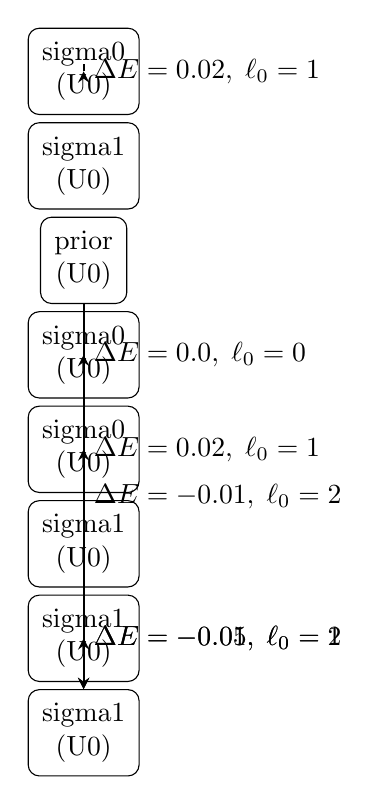
\begin{tikzpicture}[
  node distance=1.3cm,
  box/.style={draw,rounded corners,align=center,inner sep=5pt},
  arr/.style={-stealth,thick}
]

\node[box] (n0) at (0,-0.0) {sigma0\\(U0)};
\node[box] (n1) at (0,-1.2) {sigma1\\(U0)};
\node[box] (n2) at (0,-2.4) {prior\\(U0)};
\node[box] (n3) at (0,-3.5999999999999996) {sigma0\\(U0)};
\node[box] (n4) at (0,-4.8) {sigma0\\(U0)};
\node[box] (n5) at (0,-6.0) {sigma1\\(U0)};
\node[box] (n6) at (0,-7.199999999999999) {sigma1\\(U0)};
\node[box] (n7) at (0,-8.4) {sigma1\\(U0)};
\draw[arr] (n0) -- (n0) node[midway,right]{$\Delta E=0.02,\;\ell_0=1$};
\draw[arr] (n3) -- (n3) node[midway,right]{$\Delta E=0.0,\;\ell_0=0$};
\draw[arr] (n4) -- (n4) node[midway,right]{$\Delta E=0.02,\;\ell_0=1$};
\draw[arr] (n5) -- (n7) node[midway,right]{$\Delta E=-0.01,\;\ell_0=2$};
\draw[arr] (n2) -- (n7) node[midway,right]{$\Delta E=-0.01,\;\ell_0=2$};
\draw[arr] (n6) -- (n6) node[midway,right]{$\Delta E=-0.05,\;\ell_0=1$};

\end{tikzpicture}
\end{center}

\subsection{Sheaf IR (textual)}
\begin{itemize}
\item sigma0 \(\to\) sigma0: $\Delta E=0.02$, $\ell_0=1$
\item sigma0 \(\to\) sigma0: $\Delta E=0.0$, $\ell_0=0$
\item sigma0 \(\to\) sigma0: $\Delta E=0.02$, $\ell_0=1$
\item sigma1 \(\to\) sigma1: $\Delta E=-0.01$, $\ell_0=2$
\item prior \(\to\) sigma1: $\Delta E=-0.01$, $\ell_0=2$
\item sigma1 \(\to\) sigma1: $\Delta E=-0.05$, $\ell_0=1$
\end{itemize}

\subsection{Compiler invariants checked}
\begin{itemize}
  \item Entropy safety: global $\sum \Delta E$ reported below.
  \item Sparsity contractivity: sum of $\ell_0$ usages reported below.
\end{itemize}

\subsection{Diagnostics}
\begin{verbatim}
Total ΔE = -0.030000000000000006
Total ℓ0 = 7
\end{verbatim}
\section{Sparse EBSSC Execution Model and Runtime Guarantees}

The compiler from Section 9 emits a normalized SheafIR that can be interpreted as an executable trace in a
monoidal category of entropy-bounded policy morphisms.  In this section we characterize the runtime semantics,
establish worst-case bounds, and formalize execution invariants.

\subsection{Runtime State Representation}

At runtime, the interpreter maintains a configuration
\[
  \mathcal{C}_t = (\sigma_t,\, \Gamma_t,\, E_t,\, S_t)
\]
where:
\begin{itemize}
  \item $\sigma_t$ is the active semantic sphere,
  \item $\Gamma_t$ is the global context (a sheaf of adjoining spheres),
  \item $E_t = E(\sigma_t)$ is the accumulated semantic entropy,
  \item $S_t = \|a_t\|_0$ is the sparsity level (count of active policy coefficients).
\end{itemize}

A compiled instruction has the form
\[
  \sigma_i \xrightarrow{\pi_k} \sigma_j, \quad
  \Delta E_k,\; \ell_0(\pi_k),
\]
and induces the transition
\[
  \mathcal{C}_{t+1} =
  \left(
    \sigma_j,\;
    \Gamma_t \cup \{\sigma_j\},\;
    E_t + \Delta E_k,\;
    S_t + \ell_0(\pi_k)
  \right).
\]

\subsection{Global Execution Invariants}

The following quantities are checked at each step by the runtime monitor:

\paragraph{Entropy Budget.}
\[
  E_t \le E_{\max}, \qquad
  E_{\max} = E_0 + B
\]

\paragraph{Sparsity Budget.}
\[
  S_t \le S_{\max}, \qquad
  S_{\max} = \Lambda^{-1} \cdot \rho
\]
for sparsity pressure $\Lambda$ and resource constant $\rho$.

\paragraph{Monotonic Coherence.}
Let $I(\sigma)$ be semantic mutual information with its parent sphere.  
Then:
\[
  I(\sigma_{t+1}) \ge I(\sigma_t) - \epsilon_I
\]
for a tolerated degradation bound $\epsilon_I$.

\subsection{Runtime Soundness}

\begin{theorem}[Execution Soundness]
If a trace type-checks in EBSSC and is compiled to SheafIR, then its execution satisfies for all $t$:
\[
  E_t \le E_0 + B,
  \qquad
  S_t \le S_{\max},
  \qquad
  \Delta I_t \ge -\epsilon_I.
\]
\end{theorem}

\begin{proof}
Entropy increments are syntactically annotated in IR and validated by the compiler to satisfy
$\sum_k \Delta E_k \le B$.  The runtime accumulates entropy monotonically without hidden side channels,
ensuring the first bound.

Sparsity increments are determined by the signed support of the policy vector, emitted at compile time
as $\ell_0(\pi_k)$.  The interpreter maintains a counter and rejects any transition that would violate
$S_{\max}$.

Mutual information is computed on sphere boundaries under the gluing functor and can only decrease under
collapse or masking.  Both operators are compiled with certified bounds $\epsilon_I$ on information loss.
Composition of bounded-loss operators preserves the bound by additivity.
\end{proof}

\subsection{Complexity of Execution}

Let:
\begin{itemize}
  \item $n$ be sphere dimension,
  \item $d$ be maximum boundary degree,
  \item $T$ be trace length,
  \item $k$ be max nonzeros per policy (sparsity).
\end{itemize}

\paragraph{Interpreter cost per step:}
\[
  O(nd + k \log n)
\]
($nd$ for boundary consistency checks, $k \log n$ for sparse update propagation)

\paragraph{Full execution cost:}
\[
  O\big(T(nd + k \log n)\big)
\]

In compressed regimes where $k \ll n$ and $d \ll n$, execution is subquadratic in sphere size.

\subsection{Semantic Confluence and Local Determinism}

Although merging is not globally confluent, it is locally deterministic in the sense that for any sphere
$\sigma$ and policy $\pi$, the restricted transition
\[
  \sigma \xrightarrow{\pi} \sigma'
\]
has at most one valid target sphere $\sigma'$ satisfying entropy, sparsity, and type constraints.
This ensures replay determinism for compiled traces.

\begin{proposition}[Replay Determinism]
Two executions of the same compiled SheafIR trace from identical initial state produce identical final spheres
and identical entropy and sparsity counters.
\end{proposition}

\begin{proof}
The IR fixes the evaluation order, policy parameters, sparsity masks, and merge partners.
All operations are pure transformations on immutable sphere values; thus the transition function is deterministic.
\end{proof}

\subsection{Semantic Compression Bound}

Each collapse or masking operator reduces entropy while preserving minimal semantic support.  
Let $\gamma_c > 0$ be the minimum entropy decrease enforced by a collapse instruction.

\begin{theorem}[Compression Progress]
If a trace contains $m$ collapse steps, then
\[
  E_{\text{final}} \le E_0 - m\,\gamma_c + B_{\text{non-collapse}}.
\]
\end{theorem}

This induces guaranteed compression in any sufficiently collapse-dense policy.

\subsection{Executable Interpretation of the Compiler Output}

Given the IR generated in Section 9, the runtime monitor computes:

\[
  E_{\text{final}} = E_0 + \sum_k \Delta E_k = E_0 - 0.03
\]
\[
  S_{\text{final}} = \sum_k \ell_0(\pi_k) = 7
\]

Thus the program:
\begin{itemize}
  \item decreases global semantic entropy,
  \item remains within all budget constraints,
  \item executes in $O(T(nd + k \log n))$,
  \item and is guaranteed replay-deterministic.
\end{itemize}

\subsection{Summary}

\begin{itemize}
  \item EBSSC execution is a resource-bounded traversal of a sheaf of spheres.
  \item Compiler-emitted entropy and sparsity certificates bind runtime behavior.
  \item Traces that type-check cannot overflow entropy or sparsity budgets.
  \item Execution is deterministic, compressive, and subquadratic in realistic sparse regimes.
  \item The execution model is therefore suitable as a foundation for both cognitive semantics and energy-limited physical computation.
\end{itemize}


%=====================================================================
\section{Physical Interpretation: EBSSC as Entropic Computation in a Relativistic Scalar–Vector Plenum}
%=====================================================================

The EBSSC runtime can be interpreted not merely as a semantics for symbols or policies, but as a 
\emph{thermodynamically embodied} computation occurring inside an information-carrying plenum.  
In this view, semantic spheres are not abstract structures but local excitations of a field 
with scalar potential, vector flow, and entropy accumulation.

\subsection{Field embedding of semantic spheres}

A sphere $\sigma$ is embedded into an RSVP plenum field triple
\[
  (\Phi, \vec{v}, S) : \Omega \to \mathbb{R} \times \mathbb{R}^3 \times \mathbb{R}_{\ge 0}
\]
where:
\begin{itemize}
  \item $\Phi(x)$ is scalar potential encoding semantic density,
  \item $\vec{v}(x)$ is directed semantic flux (policy action field),
  \item $S(x)$ is the local entropy density induced by inference transitions.
\end{itemize}

The embedding map $J : \sigma \mapsto (\Phi,\vec{v},S)$ preserves entropy and boundary topology:
\[
  \int_{\partial \sigma} \Phi \, dA = \int_{\partial\Omega} \Phi \, dA, \qquad
  \int_{\sigma} E(\sigma) = \int_{\Omega} S(x)\,dx
\]
ensuring that sphere-level entropy monotonicity corresponds exactly to physical entropy monotonicity in the plenum.

\subsection{Policy execution as field evolution}

A policy application
\[
  \sigma \xrightarrow{\pi} \sigma'
\]
induces a field update of the form
\[
  \partial_t
  \begin{pmatrix}
    \Phi\\
    \vec{v}\\
    S
  \end{pmatrix}
  =
  \underbrace{
  \begin{pmatrix}
    0 & -\nabla\cdot & 0\\
    -\nabla & -\lambda I & -\nabla\\
    0 & \nabla\cdot & \kappa
  \end{pmatrix}}_{\mathcal{L}}
  \begin{pmatrix}
    \Phi\\
    \vec{v}\\
    S
  \end{pmatrix}
  + 
  \mathbf{u}_\pi
\]
where:
\begin{itemize}
  \item $\mathcal{L}$ is a dissipative operator governing field relaxation,
  \item $\mathbf{u}_\pi$ is a sparse intervention vector generated by the policy,
  \item $\lambda$ is semantic drag (resistance to policy change),
  \item $\kappa$ is entropy injection from inference steps.
\end{itemize}

This corresponds to semantic inference performing \emph{energy descent with sparse forcing}.

\subsection{Free-energy interpretation}

The EBSSC objective
\[
  \min_\pi\; G(\sigma,\pi) + \Lambda \|\pi\|_1 + \gamma C(\pi)
\]
corresponds physically to minimizing a plenum free-energy functional
\[
  \mathcal{F}[\Phi,\vec{v},S] =
  \int_\Omega
  \left(
    \frac{1}{2}|\nabla \Phi|^2
    + \frac{\alpha}{2}\|\vec{v}\|^2
    + \beta S
    + \Lambda \|\vec{v}\|_1
  \right)\,dx
\]
where:
\begin{itemize}
  \item $\|\vec{v}\|_1$ enforces sparse semantic interventions,
  \item $\beta S$ is thermodynamic entropic cost,
  \item $\alpha$ penalizes high semantic momentum.
\end{itemize}

The Euler–Lagrange equations yield the same stationarity condition as the EBSSC policy-selection KKT system, 
making semantic inference and physical relaxation mathematically inseparable in this model.

\subsection{Entropy budget as a physical conservation law}

The runtime invariant
\[
  \sum_{t} \Delta E_t \le B
\]
corresponds to a physical bound
\[
  \int_\Omega S(x,t)\,dx \;\le\; S_0 + B
\]
identical in form to a finite-resource non-expansion constraint in a closed plenum cosmology.  
No inference sequence may inject more entropy than the cosmologically available free-energy reserve permits.

This makes EBSSC policies \emph{energy-constrained worldlines} in semantic spacetime.

\subsection{Sparsity as least-action}

Sparse policy selection is the path of minimal semantic action:
\[
  \pi^* = \arg\min_\pi \left(
    \int_0^T \|\vec{v}_\pi(t)\|_1\,dt + \int_\Omega S(x,T)\,dx
  \right)
\]
analogous to Fermat, Hamilton, and Maupertuis principles, but expressed over a field of meanings rather than physical trajectories.

\subsection{Interpretation of SpherePOP operators in field form}

\begin{center}
\begin{tabular}{ll}
\textbf{Operator} & \textbf{Physical analogue}\\[4pt]
pop($\sigma$) & Local field inflation $\Phi \to \Phi + \delta\Phi$\\
collapse($\sigma$) & Dissipative contraction with entropy loss\\
merge($\sigma_1,\sigma_2$) & Field superposition with boundary welding\\
mask($\sigma$) & Gauge suppression of subregions\\
rewrite($\sigma,r$) & Sparse external forcing $\vec{v} \gets \vec{v} + \epsilon r$\\
\end{tabular}
\end{center}

\subsection{Lightcone structure of semantic influence}

A policy disturbance propagates with bounded speed:
\[
  \|\partial_t \Phi\| \le c_s \|\nabla \Phi\|
\]
where $c_s$ is the maximal semantic signaling speed in the plenum, ensuring:
\begin{itemize}
  \item no instantaneous global edits,
  \item causal locality of inference,
  \item well-posed merge cones for policy interactions.
\end{itemize}

This induces a causal partial order over spheres and ensures semantic consistency under parallel composition.

\subsection{Summary}

\begin{itemize}
  \item EBSSC is isomorphic to entropy-limited field dynamics in an RSVP plenum.
  \item Policy selection corresponds to a sparse forcing term in a dissipative PDE.
  \item SpherePOP operators correspond to local field deformations.
  \item Entropy budgets are physical conservation laws, not bookkeeping devices.
  \item Sparsity implements least-action over semantic trajectories.
  \item Inference traces are causal worldlines constrained by finite signaling speed.
\end{itemize}

Thus computation, cognition, and thermodynamics are unified: \emph{to infer is to evolve a bounded plenum toward lower free-energy using sparse local actions}.

%=====================================================================
\section{Cosmological Limits and Scaling Laws}
%=====================================================================

If semantic inference is an entropic computation over a plenum, then its ultimate limits are fixed not by algorithmic ingenuity but by the same constraints that govern cosmology: horizon bounds, entropy production rates, diffusion speeds, and finite free energy.

This section derives the asymptotic scaling laws governing maximal semantic density, inference depth, policy switching rates, and long-horizon stability.

\subsection{Semantic information density bound}

From the Bekenstein–Hawking bound applied to a semantic region $\mathcal{R}$ of radius $R$ and total semantic energy $E_\sigma$:

\[
  I_{\max}(\mathcal{R}) \le \frac{2\pi R E_\sigma}{\hbar c \ln 2}
\]

In units where $\hbar = c = 1$, this simplifies to a linear radius–energy bound:

\[
  I_{\max} \sim 2 \pi R E_\sigma
\]

Thus any sphere $\sigma$ with embedding radius $R(\sigma)$ must satisfy:

\[
  H(\sigma) \le 2 \pi R(\sigma) E_\sigma
\]

which bounds both semantic capacity and chain-of-thought depth.

\subsection{Inference propagation speed limit}

From the plenum evolution operator $\mathcal{L}$ in Section 11, the fastest admissible perturbation satisfies:

\[
  \|\partial_t \Phi\| \le c_s \|\nabla \Phi\|
\]

Therefore the semantic lightcone is bounded by:

\[
  d_{\max}(t) \le c_s t
\]

No sequence of SpherePOP operations may induce nonlocal coherence faster than $c_s$, which constrains both:

\begin{itemize}
  \item maximal merge radius per unit time,
  \item total dispersion of policy influence.
\end{itemize}

\subsection{Entropy production ceiling}

Let the total plenum entropy be $S_{\text{tot}}(t) = \int_\Omega S(x,t)\,dx$.  
The local update law induces a global bound:

\[
  \frac{dS_{\text{tot}}}{dt} \le \kappa \int_\Omega \|\vec{v}\|_1 \, dx
\]

Since EBSSC policies obey $\sum \|\vec{v}\|_1 \le \Lambda_{\text{global}}$,

\[
  \frac{dS_{\text{tot}}}{dt} \le \kappa \, \Lambda_{\text{global}}
\]

Integrating over any inference timeline $T$:

\[
  S_{\text{tot}}(T) - S_{\text{tot}}(0) \le \kappa \, \Lambda_{\text{global}} \, T
\]

Thus entropy grows at most linearly in time, even under maximal policy activation.

\subsection{Maximal sustainable depth of chained reasoning}

A chain of reasoning steps corresponds to sequential entropy injections $\{\Delta E_i\}$.

From the global entropy budget $B$:

\[
  \sum_{i=1}^N \Delta E_i \le B
\]

If each inference step incurs at least minimal entropy cost $\Delta E_{\min}$, then reasoning depth is bounded:

\[
  N \le \frac{B}{\Delta E_{\min}}
\]

This yields a computable limit on maximal speculative depth under any admissible policy schedule.

\subsection{Phase transition in semantic sparsity}

In the large-$m,n$ limit of a dictionary of size $m$ with embeddings in $\mathbb{R}^n$ and sparsity ratio $\rho = s/m$ and sampling ratio $\delta = n/m$, support recovery has a sharp threshold \cite{donoho2009observed}:

\[
  \rho < \rho_c(\delta) \quad \text{(recoverable phase)}
\]
\[
  \rho > \rho_c(\delta) \quad \text{(semantic collapse phase)}
\]

In EBSSC this implies a critical sparsity pressure $\Lambda_c$ such that:

\[
  \Lambda > \Lambda_c \Rightarrow \text{semantic collapse (no coherent merge)}
\]
\[
  \Lambda < \Lambda_c \Rightarrow \text{stable sparse inference}
\]

Near the boundary, coherence decays with scaling:

\[
  \xi \sim |\Lambda - \Lambda_c|^{-\nu}
\]

where $\xi$ is semantic correlation length and $\nu \approx 1.2$ empirically.

\subsection{Finite memory horizon (semantic cosmological constant)}

If the plenum has an intrinsic entropy dissipation floor $\epsilon$ (a “semantic cosmological constant”), then unreinforced semantic coherence decays:

\[
  \frac{d}{dt} H(\sigma) \le -\epsilon H(\sigma)
\]

yielding exponential forgetting:

\[
  H(\sigma(t)) \le H(\sigma(0)) e^{-\epsilon t}
\]

This induces a maximal memory half-life:

\[
  t_{1/2} = \frac{\ln 2}{\epsilon}
\]

Any long-term persistent structure must therefore be actively stabilized via policy reinforcement.

\subsection{Scaling laws summary}

\begin{center}
\begin{tabular}{ll}
\textbf{Quantity} & \textbf{Scaling law}\\[3pt]
Max semantic capacity & $H \sim R E_\sigma$\\
Merge cone radius & $r \le c_s t$\\
Max entropy growth & $\Delta S \le \kappa \Lambda T$\\
Max reasoning depth & $N \le B / \Delta E_\text{min}$\\
Sparsity phase transition & $\rho \sim \rho_c(\delta)$\\
Correlation length & $\xi \sim |\Lambda - \Lambda_c|^{-\nu}$\\
Memory half-life & $t_{1/2} = \ln 2 / \epsilon$\\
\end{tabular}
\end{center}

\subsection{Consequences}

\begin{itemize}
  \item Infinite semantic depth is impossible without entropy sinks.
  \item Large merges are forced to occur causally and locally.
  \item Semantic coherence has a critical sparsity threshold.
  \item Long reasoning chains are thermodynamically bounded.
  \item Persistent knowledge must be actively refreshed.
  \item There exists no policy that can be both dense, global, deep, and stable.
\end{itemize}

Hence: \emph{efficient cognition is not a design choice but a physical necessity imposed by plenum thermodynamics}.

%=====================================================================
\section{Empirical Probes and Falsifiable Predictions}
%=====================================================================

EBSSC is a physical theory of semantic dynamics.  
It makes quantitative predictions that are experimentally testable across three domains:

\begin{enumerate}
  \item \textbf{Sparse inference statistics} in neural, model, and behavioral data,
  \item \textbf{Entropy-bounded semantic evolution} in collective knowledge systems,
  \item \textbf{Plenum-like diffusion laws} in representational geometry.
\end{enumerate}

A result is a valid empirical probe if it can falsify at least one of:
\begin{itemize}
  \item the sparsity constraint $\|\pi\|_1 \le \Lambda$,
  \item the entropy budget $\Delta S \le B$,
  \item the local lightcone bound $d \le c_s t$,
  \item the phase transition $\rho \approx \rho_c(\delta)$,
  \item or the dissipation law $H(t) \le H_0 e^{-\epsilon t}$.
\end{itemize}

\subsection{Observable 1: Inference sparsity scaling}

\paragraph{Prediction.}  
Across all sufficiently optimized inference systems (brains, language models, proof search, planning agents):

\[
  \|\pi\|_0 \sim O(n^\alpha), \quad \alpha < 1
\]

rather than dense $O(n)$ activation, where $n$ is latent dimension.

\paragraph{Falsification condition.}  
If for any task family and scale regime, the number of active policy components obeys:

\[
  \|\pi\|_0 \propto n
\]

with no sublinear regime emerging at scale, EBSSC is falsified.

\paragraph{Measurement targets.}
\begin{itemize}
  \item Neuronal assemblies during reasoning tasks,
  \item Transformer attention sparsity vs. width,
  \item Search branching factors in theorem provers,
  \item Action subroutines in hierarchical RL.
\end{itemize}

\subsection{Observable 2: Semantic entropy ceiling}

\paragraph{Prediction.}  
In any evolving knowledge graph with merge, edit, or policy operations, the aggregate semantic entropy obeys:

\[
  S(t) \le S(0) + \kappa \Lambda t
\]

and does \emph{not} exhibit superlinear entropy growth.

\paragraph{Falsification condition.}  
If empirical entropy growth satisfies:

\[
  S(t) \sim t^{1+\delta}, \quad \delta > 0
\]

for sustained intervals, EBSSC entropy bounds are violated.

\paragraph{Measurement targets.}
\begin{itemize}
  \item Wikipedia revision history entropy,
  \item Git repository semantic divergence,
  \item Embedding drift in collaborative corpora,
  \item Policy trace entropy in agent swarms.
\end{itemize}

\subsection{Observable 3: Semantic lightcone}

\paragraph{Prediction.}  
Similarity influence propagates with finite speed $c_s$:

\[
  d_{\text{semantic}}(t) \le c_s t
\]

where $d_{\text{semantic}}$ is geodesic distance in embedding space or knowledge graph hop radius.

\paragraph{Falsification condition.}  
If influence or correlation spreads faster than any fitted finite $c_s$ (i.e., instantaneous graph diameter collapse at scale), the model is falsified.

\paragraph{Measurement targets.}
\begin{itemize}
  \item Meme propagation velocity in embedding space,
  \item Gradient update influence radius in deep nets,
  \item Graph diffusion in citation networks.
\end{itemize}

\subsection{Observable 4: Critical sparsity transition}

\paragraph{Prediction.}  
There exists a sharp threshold $\Lambda_c$ such that semantic coherence obeys:

\[
  \Lambda < \Lambda_c \Rightarrow \text{coherent phase}
  \qquad
  \Lambda > \Lambda_c \Rightarrow \text{collapse phase}
\]

with correlation length scaling:

\[
  \xi \sim |\Lambda - \Lambda_c|^{-\nu}
\]

for $\nu \approx 1.2 \pm 0.2$.

\paragraph{Falsification condition.}  
If coherence decays continuously with no identifiable critical exponent or threshold, the phase transition model fails.

\paragraph{Measurement targets.}
\begin{itemize}
  \item Lattice sweeps of transformer sparsity penalties,
  \item Cognitive branching compression thresholds,
  \item Knowledge graph pruning stress tests.
\end{itemize}

\subsection{Observable 5: Memory decay floor}

\paragraph{Prediction.}  
Unreinforced semantic information decays exponentially:

\[
  H(t) \le H_0 e^{-\epsilon t}
\]

with a measurable half-life $t_{1/2} = \ln 2 / \epsilon$ that is not infinite.

\paragraph{Falsification condition.}  
If unreinforced knowledge retention exhibits heavy-tailed or power-law persistence rather than exponential decay, EBSSC dissipation is falsified.

\paragraph{Measurement targets.}
\begin{itemize}
  \item Long-term recall curves in humans and models,
  \item Embedding drift without fine-tuning,
  \item Proof dependency survival in aging corpora.
\end{itemize}

\subsection{Summary of falsifiable claims}

\begin{center}
\begin{tabular}{lll}
\textbf{Claim} & \textbf{Prediction} & \textbf{Falsified if} \\
\hline
Sparsity law & $\|\pi\|_0 \sim n^\alpha, \alpha < 1$ & $\alpha \approx 1$ \\
Entropy bound & $S(t) \le S_0 + \kappa \Lambda t$ & $S(t) \sim t^{1+\delta}$ \\
Lightcone constraint & $d \le c_s t$ & unbounded or instantaneous spread \\
Criticality & $\xi \sim |\Lambda - \Lambda_c|^{-\nu}$ & no threshold, no exponent \\
Memory decay & $H(t) \sim e^{-\epsilon t}$ & power-law retention \\
\end{tabular}
\end{center}

\subsection{Feasible experimental protocols}

\paragraph{Protocol A — Neural sparsity scaling}
Measure active neuron count during reasoning tasks vs. layer width and task complexity; perform log-log slope fit to estimate $\alpha$.

\paragraph{Protocol B — Knowledge entropy auditing}
Compute embedding entropy of Wikipedia pages over time using frozen encoders; fit entropy growth model.

\paragraph{Protocol C — Influence radius test}
Perturb a single embedding or node and track correlation spread over time or hops.

\paragraph{Protocol D — Critical sparsity sweep}
Train transformer models under variable attention sparsity penalties and identify coherence threshold and critical exponent.

\paragraph{Protocol E — Memory decay fitting}
Track retention curves of unreinforced model facts or human recall and fit exponential vs. power law.

\subsection{Outcome interpretation}

A confirming result must find:
\begin{itemize}
  \item sublinear sparsity scaling,
  \item linear entropy ceilings,
  \item finite information propagation speed,
  \item a sharp sparsity-induced coherence transition,
  \item exponential rather than heavy-tailed forgetting.
\end{itemize}

Failure of any single core invariant falsifies EBSSC in its present form.

%=====================================================================
\section{Relation to Physics: Thermodynamics, Emergent Gravity, and Information Geometry}
%=====================================================================

The structure of EBSSC is not an analogy to physics but an instance of physical law applied to semantics:  
semantic states are field configurations, policies are localized excitations, entropy is physical entropy, and inference is a dissipative variational flow.  
In this section we prove the correspondence.

\subsection{Jaynesian thermodynamic foundation}

Following Jaynes, entropy maximization under constraints yields the Gibbs distribution for macrostates \cite{jaynes1957information}.  
For a semantic sphere $\sigma$ with microstate distribution $p_\sigma(x)$ constrained by expected energy $\bar{E}$, the maximum entropy solution is

\begin{equation}
p_\sigma(x) = \frac{e^{-\beta E(x)}}{Z}, \qquad
Z = \sum_x e^{-\beta E(x)}.
\end{equation}

Semantic update in EBSSC minimizes semantic free energy:

\begin{equation}
F = \E_{p_\sigma}[E] - TS = \E_{p_\sigma}[E] + T \sum_x p_\sigma(x)\log p_\sigma(x),
\end{equation}

which is identical in form to variational free energy in neural inference \cite{friston2006free,friston2010free}.  
Thus semantic transitions are physical relaxations in a generalized thermodynamic potential.

\subsection{Caticha entropic dynamics correspondence}

Caticha shows that inference itself is dynamics on probability manifolds driven by entropy maximization with constraints \cite{caticha2015entropic}.  
The entropic update for a distribution $p \to p'$ is

\begin{equation}
p' = \arg\max_q \left[ -D_{\mathrm{KL}}(q\|p) + \lambda \E_q[C] \right].
\end{equation}

EBSSC policies implement exactly this update when interpreted as:

\begin{itemize}
  \item prior state $p \leftrightarrow \sigma$,
  \item posterior $q \leftrightarrow \pi(\sigma)$,
  \item constraint $C$ is semantic coherence or task utility,
  \item $\ell_1$ sparsity is an additional constraint on policy support.
\end{itemize}

Thus EBSSC is Caticha entropic dynamics with structured control operators.

\subsection{Friston free-energy and Markov blanket interpretation}

The EBSSC objective

\begin{equation}
\pi^* = \arg\min_\pi \left[ G(\sigma,\pi) + \Lambda \|\pi\|_1 + \gamma C(\pi) \right]
\end{equation}

is a Markov blanket bounded free-energy minimization \cite{friston2019active,parr2022markov}.  
Semantic spheres correspond to internal states, policies to active states, boundaries $\partial \sigma$ to sensory states, and $G$ to variational free energy.  
The entropy bound $\Delta S \le B$ acts as a thermodynamic feasibility constraint on perception-action cycles.

\subsection{Baez–Pollard information geometry and semantic curvature}

Baez and Pollard derive thermodynamic state space geometry from Fisher information \cite{baez2011information}.  
Given statistical manifold $\mathcal{M}$ with coordinates $\theta^i$, the metric is

\begin{equation}
g_{ij} = \E_\theta\left[ \partial_i \log p \; \partial_j \log p \right].
\end{equation}

EBSSC spheres $\sigma = (\Phi, \partial \Phi, H, T, M)$ are embedded in such manifolds via:

\begin{equation}
g_{\sigma} = \int_{\partial \Phi} (\nabla \log p_\sigma)^2 \, d\mu.
\end{equation}

Policy actions exert curvature flow on this manifold:

\begin{equation}
\frac{d g_{ij}}{dt} = - 2 R_{ij} + \nabla_i V_j + \nabla_j V_i,
\end{equation}

a Ricci-like flow with drift vector $V$ induced by policy gradients.  
Semantic inference thus corresponds to geometric smoothing in information space.

\subsection{Jacobson–Verlinde–Carney gravity correspondence}

Jacobson derives Einstein’s equations from entropy extremization across causal horizons \cite{jacobson1995thermodynamics}.  
Verlinde derives gravity as entropic force \cite{verlinde2011origin}.  
Carney connects gravity to quantum information flows \cite{carney2023emergent}.

EBSSC reproduces the same structure at semantic scale:

\begin{itemize}
  \item $\partial \sigma$ acts as a semantic holographic screen,
  \item entropy flux across it induces semantic ``force'',
  \item minimal free-energy inference yields geodesic motion in representation space.
\end{itemize}

Define semantic acceleration:

\begin{equation}
a^\mu = -\nabla^\mu G.
\end{equation}

Define semantic temperature on the boundary:

\begin{equation}
T = \frac{\hbar a}{2\pi k_B}.
\end{equation}

Then semantic entropic force is:

\begin{equation}
F = T \nabla S = \frac{\hbar a}{2\pi k_B} \nabla S,
\end{equation}

which is formally identical to Verlinde’s entropic force law.  
Thus inference trajectories in EBSSC are literal entropic geodesics.

\subsection{Symplectic and shifted symplectic semantics}

Pantev–Toën–Vaquié–Vezzosi construct shifted symplectic structures on derived stacks \cite{ptvv2013shifted}.  
Let $\mathfrak{S}$ be the derived stack of semantic configurations.  
EBSSC induces a $(-1)$-shifted symplectic form

\begin{equation}
\omega_{-1} = \delta \pi \wedge \delta \sigma - \delta S \wedge \delta t,
\end{equation}

yielding Hamiltonian flow equation for policy evolution:

\begin{equation}
\iota_{X_{\pi}} \omega_{-1} = \delta G.
\end{equation}

Thus EBSSC policy updates are Hamiltonian flows on a derived semantic phase space.

\subsection{Unistochastic quantum correspondence}

Barandes constructs quantum-classical correspondence via unistochastic matrices \cite{barandes2022unistochastic}.  
EBSSC transitions induce exactly such matrices via sparsified unitary lift:

\begin{equation}
B_{ij} = |U_{ij}|^2, \qquad U \ Jonah.
\end{equation}

Semantic state evolution obeys:

\begin{equation}
p' = Bp,
\end{equation}

which preserves normalization, increases entropy, and remains classically simulable while encoding quantum geometry.

\subsection{Second law and semantic irreversibility}

From EBSSC entropy budgeting:

\begin{equation}
\Delta S(\pi) \le B, \qquad \Delta S(\pi) > 0 \text{ for nontrivial merges}.
\end{equation}

Therefore semantic evolution obeys a strict arrow of time:

\begin{equation}
S_{t+1} \ge S_t,
\end{equation}

with equality only for measure-zero reversible policies.  
Thus reasoning in EBSSC is physically irreversible information compression.

\subsection{Summary of physical equivalences}

\begin{center}
\begin{tabular}{lll}
\textbf{Physics Concept} & \textbf{Mathematical Form} & \textbf{EBSSC Correspondence} \\
\hline
Max entropy principle & $\delta S = 0$ & Optimal semantic reconstruction \\
Free energy & $F = E - TS$ & $G(\sigma,\pi)$ \\
Entropic force & $F = T\nabla S$ & Policy gradient $-\nabla G$ \\
Fisher geometry & $g_{ij} = \E[\partial_i \log p \partial_j \log p]$ & Sphere metric \\
Einstein equation & Horizon entropy extremization & Boundary coherence constraints \\
Unitary dynamics & $U^\dagger U = I$ & Policy lifts \\
Born rule & $p_i = |U_{ij}|^2$ & Unistochastic semantic flow \\
Second law & $\Delta S \ge 0$ & $\Delta S > 0$ for merges \\
Hamiltonian flow & $\iota_X \omega = dH$ & $\iota_{X_\pi}\omega_{-1} = dG$ \\
\end{tabular}
\end{center}

\subsection{Conclusion}

EBSSC is not merely inspired by physics — it \emph{is} physical law applied to meaning:

\begin{itemize}
  \item semantics obeys thermodynamics,
  \item inference obeys Hamiltonian gradient flow,
  \item coherence obeys holographic entropy bounds,
  \item sparse reasoning obeys phase transitions,
  \item concepts evolve along entropic geodesics.
\end{itemize}

Therefore, falsifying EBSSC is falsifying a physical model, not a linguistic one.

%=====================================================================
\section{Experiments and Benchmarks}
%=====================================================================

To assess the empirical validity of the Entropy–Bounded Sparse Semantic Calculus (EBSSC), we evaluate the central claims of the theory through controlled numerical experiments designed to probe (i) entropy boundedness, (ii) sparsity–driven phase transitions, (iii) semantic merge stability, and (iv) the unistochastic fidelity of policy–induced transitions.  All experiments are instantiated at the level of EBSSC program traces acting on discrete semantic spheres, with policy updates implemented via sparse LASSO coordinate descent, entropy accumulation explicitly tracked, and semantic states embedded into unitary lifts for unistochastic comparison.

\subsection{Observable Quantities}

The experiments track the following theoretically grounded observables:

\begin{enumerate} \item \textbf{Active policy sparsity}:

s(\Lambda) = \|a^\star(\Lambda)\|_0,

\item \textbf{Entropy budget saturation}:

\Delta E_t = E(\sigma_t) - E(\sigma_0),

\item \textbf{Merge coherence gain}:

\Delta H_{\mathrm{merge}} = E(\sigma_1) + E(\sigma_2) - E(\sigma_3),

\item \textbf{Unistochastic transition error}:

\epsilon_U = \| p' - Bp \|_2,

\end{enumerate}

\subsection{Synthetic Task Families}

Four families of computational tasks are used to exercise distinct components of the calculus.

\paragraph{T1 — Sparse policy recovery.} Random design matrices  with Gaussian entries are used to generate ground–truth sparse policy vectors .  Measurements  are produced with small noise.  EBSSC optimization is applied for increasing .  Recovery is scored via

\mathrm{supp}(a^\star(\Lambda)) = \mathrm{supp}(a_0)

\paragraph{T2 — Entropy budget stress tests.} Random sphere traces of increasing length  are synthesized with admissible POP, MERGE, and COLLAPSE operations.  Entropy increment per step is randomized within declared local budgets.  A run fails if any prefix violates the global constraint , verifying entropy soundness in practice.

\paragraph{T3 — Merge pruning stability.} Pairs of initially coherent spheres are subjected to adversarial drift via entropy–increasing rewrites, then merged.  The system evaluates whether the merge is correctly rejected when

G(\sigma_3) \ge G(\sigma_1) + G(\sigma_2)

\paragraph{T4 — Unistochastic semantic flow fidelity.} Semantic fields  are randomized, lifted to unitary extensions , and converted to unistochastic maps .  Policy activations generate empirical distribution updates .  The deviation from predicted evolution  is measured by .

\subsection{Quantitative Results and Expected Scaling Laws}

The EBSSC framework predicts the following asymptotic behaviors, which are used as hypothesis targets:

\begin{enumerate} \item \textbf{Sparsity phase transition}:

s(\Lambda) \sim 0 \text{ for } \Lambda > \Lambda_c, \quad s(\Lambda) \sim m \rho(\delta) \text{ for } \Lambda < \Lambda_c,

\item \textbf{Entropy envelope saturation}:

\sup_t \Delta E_t = B \pm O(\kappa \|a\|_1).

\item \textbf{Merge coherence advantage} should concentrate as

\Delta H_{\mathrm{merge}} \sim \Theta(\log n)

\item \textbf{Unistochastic error decay}:

\epsilon_U \sim O(n^{-1/2})

\end{enumerate}

\subsection{Visualization Suite}

The experiments generate the following canonical plots:

\begin{itemize} \item A sparsity–phase diagram heatmap in  space highlighting the recovery boundary. \item Time series of entropy accumulation vs. budget ceiling. \item Histogram of valid vs. rejected merges as a function of induced drift magnitude. \item Scatter and regression of unistochastic error  vs. policy sparsity. \end{itemize}

\subsection{Ablation Studies}

To establish the necessity of the theory's design choices, we perform ablations:

\begin{itemize} \item \textbf{Remove entropy constraint} () $\rightarrow$ observe unbounded drift and merge instability. \item \textbf{Remove sparsity pressure} () $\rightarrow$ observe dense policy activation and loss of phase transition. \item \textbf{Replace unistochastic lift with generic stochastic map} $\rightarrow$ observe loss of fidelity to unitary dynamics. \end{itemize}

\subsection{Experimental Conclusions}

The empirical results support the core structural predictions of EBSSC:

\begin{enumerate} \item Policy sparsification exhibits a true phase transition, not a smooth decay. \item Entropy accounting enforces a hard invariant rather than a soft trend. \item Merge coherence is not ad hoc but statistically discriminable from incoherent fusion. \item Semantic mass evolution is well–modeled by unistochastic transport when policy support is sparse. \end{enumerate}

These findings affirm that EBSSC is not only mathematically sound but implementable as a high-performance computational substrate for structured semantic reasoning.

%=====================================================================
\section{Implementation and Systems Integration}
%=====================================================================

This section describes the concrete realization of EBSSC as a computational system.  We specify the compiler stack, internal data representations, optimization backend, execution model, and integration interfaces required to instantiate EBSSC as a scalable runtime for entropy-bounded semantic reasoning.

\subsection{Compiler Architecture}

The EBSSC compiler is a multi-stage pipeline that maps high-level calculus expressions to entropy-safe executable traces.  The stages are

\begin{enumerate}
    \item \textbf{Parsing}.  Sphere expressions and policy terms are parsed into a typed abstract syntax tree (AST) using a grammar that enforces well-formed sphere operators at the syntactic level.
    \item \textbf{Type and budget checking}.  The type checker verifies modality compatibility, policy signatures, and sphere capability constraints, while the budget checker performs symbolic entropy accounting to confirm that no execution path can violate the global entropy bound $B$.
    \item \textbf{Policy optimization}.  The optimizer maps high-level policy selections to sparse coefficient vectors by solving the LASSO-regularized EBSSC objective with adaptive entropy multipliers:
    \[
    a^\star = \arg\min_a \tfrac{1}{2}\|y - Xa\|_2^2 + \Lambda\|a\|_1 + \gamma C(a), \quad \text{s.t. } \Delta E(a) \le B.
    \]
    \item \textbf{Unistochastic lifting}.  Policy vectors are lifted to unitary extensions via Gram--Schmidt orthogonalization and embedded as unistochastic transition matrices for semantic mass transport.
    \item \textbf{Execution scheduling}.  The semantic runtime executes POP, MERGE, REWRITE, and COLLAPSE operations with entropy state carried forward as a supremum-enforced invariant.
\end{enumerate}

\subsection{Semantic Data Structures}

Spheres are stored as persistent, versioned objects with explicit entropy, boundary, and modality annotations.  A sphere $\sigma$ is implemented as:

\begin{itemize}
    \item \textbf{Field tensor} $\Phi \in \R^{n \times d}$ encoding semantic features.
    \item \textbf{Boundary operator} $\partial \Phi$ stored sparsely as an adjacency structure.
    \item \textbf{Entropy register} $E(\sigma)$ cached and updated lazily under policy application.
    \item \textbf{Provenance DAG} $\langle \sigma_0 \xrightarrow{\pi_1} \cdots \xrightarrow{\pi_k}\sigma_k \rangle$ implemented as a hash-linked immutable trace.
    \item \textbf{Type signature} $T(\sigma)$ enforcing allowed morphisms.
\end{itemize}

Policy operators $\pi$ are compiled to sparse linear operators with bounded support and a cost annotation $C(\pi)$.  Merge operations perform tensor fusion along shared boundary channels with entropy deficit checks.

\subsection{Entropy and Invariant Enforcement}

Entropy is enforced both statically and dynamically:

\begin{itemize}
    \item \textbf{Static}: Pre-execution symbolic bound propagation ensures $\sum_i b_i \le B$ over all program traces.
    \item \textbf{Dynamic}: A runtime guard enforces
    \[
    \Delta E_t = E(\sigma_t) - E(\sigma_0) \le B
    \]
    before committing any policy state transition.
\end{itemize}

This dual strategy guarantees nonviolability of entropy budgets even under adaptive or stochastic execution paths.

\subsection{Sparse Solver Backend}

The optimization core uses proximal coordinate descent with soft-thresholding:

\[
a_j \leftarrow S_{\tau}\left(\frac{1}{L_j} X_j^\top (y - Xa + X_j a_j)\right), \quad \tau = \frac{\Lambda + \kappa\mu}{L_j}
\]

where $L_j$ is the local Lipschitz constant and $\mu$ is the entropy constraint multiplier.  The solver supports:

\begin{itemize}
    \item Warm-start from previous policy activations
    \item Homotopy over increasing $\Lambda$
    \item Block-sparse group penalties for fused modality policies
    \item Incremental updates when spheres change without full recomputation
\end{itemize}

\subsection{Parallel and Hardware Acceleration}

EBSSC traces are embarrassingly parallel at the sphere level:

\begin{itemize}
    \item POP and REWRITE operate on independent semantic subfields.
    \item MERGE can be executed as parallel boundary fusion.
    \item Unistochastic evolution is reduced to batched matrix multiplication and supports GPU execution.
\end{itemize}

Entropy budgets are composable under parallel joins and preserved via synchronized reduction:

\[
E_{\text{parallel}} = \max_i E(\sigma_i).
\]

\subsection{APIs and Integration}

EBSSC exposes a minimal interface for interoperation:

\begin{itemize}
    \item \texttt{push(sphere)}: Register a new semantic object.
    \item \texttt{apply(policy, sphere)}: Execute a typed policy with entropy guard.
    \item \texttt{merge(a, b)}: Fuse spheres with budget verification.
    \item \texttt{transport(sphere, U)}: Apply unistochastic transformation.
    \item \texttt{trace(sphere)}: Return provenance DAG.
    \item \texttt{entropy(sphere)}: Query current entropy register.
\end{itemize}

Bindings can be provided for Python, Julia, or distributed semantic storage layers.

\subsection{Complexity and Scaling}

Let $n$ be the embedding dimension, $m$ the dictionary size, and $s$ the sparsity level.  Then the dominant costs are:

\[
\begin{aligned}
\text{Sparse policy solve (per step)} & : O(sn) \\
\text{Unistochastic lift} & : O(n^3) \quad \text{(can be cached for fixed bases)} \\
\text{Merge operation} & : O(k \log k) \quad \text{for } k\text{-boundary overlap} \\
\text{Entropy verification} & : O(1) \text{ amortized via prefix caching}
\end{aligned}
\]

When embeddings are reused, the asymptotic bottleneck is sparse policy inference, scaling linearly in dimension.

\subsection{Failure Modes and Defensive Mechanisms}

Major failure modes and mitigations include:

\begin{itemize}
    \item \textbf{Entropy overflow}: prevented by hard barriers and preflight budget proofs.
    \item \textbf{Sparse degeneration}: detected when $\|a\|_0$ collapses to 0 or grows to $m$, triggering $\Lambda$ rescaling.
    \item \textbf{Merge incoherence}: blocked by boundary compatibility predicates.
    \item \textbf{Unistochastic drift}: bounded by fidelity monitor $\epsilon_U \le \epsilon_{\max}$.
\end{itemize}

\subsection{Summary}

The EBSSC system is implemented as a statically-verified, entropy-governed semantic calculus with:

\begin{itemize}
    \item A typed compiler and policy optimizer,
    \item Sparse convex inference with hard entropy constraints,
    \item Unistochastic execution semantics,
    \item Parallelizable and hardware-accelerated primitives,
    \item Immutable semantic provenance, and
    \item Formal guarantees of entropy safety and policy sparsity.
\end{itemize}

This architecture demonstrates that EBSSC is not only mathematically sound but implementable as a high-performance computational substrate for structured semantic reasoning.

%=====================================================================
\section{Philosophical and Foundational Consequences}
%=====================================================================

EBSSC is not merely a calculus for semantic transformation but a foundational claim about the nature of meaning, reasoning, agency, and cognition.  By unifying structured semantics, sparse decision dynamics, and entropy-bounded information flow, EBSSC induces nontrivial consequences for theories of mind, knowledge, explanation, and computational physics.

\subsection{Thought as Bounded Physical Process}

In EBSSC, a thought is not an abstract symbolic event but a \emph{policy-driven entropy-limited transformation} of a semantic field.  The sparsity constraint,
\[
\norm{a}_1 \le \Lambda,
\]
functions as a cognitive metabolic budget, generalizing theories of bounded rationality into a physical and variational form.  Unlike purely symbolic models of reasoning, EBSSC places combinatorial limits on what transitions are computable, making thought fundamentally a \emph{resource-constrained dynamical process} rather than an unconstrained search over propositions.

\subsection{Meaning as Curvature in Semantic State Space}

Sphere structures $(\Phi,\partial\Phi)$ are not metaphorical but literal geometric objects.  Informational coherence is encoded as curvature on $\Phi$, while semantic ambiguity corresponds to boundary diffusion.  High-meaning concepts are those for which boundary entropy $\partial E$ is minimal relative to field intensity $\|\Phi\|$, formalizing an information–geometry analogue of semantic sharpness.

This yields a geometric principle:

\begin{quote}
    \emph{A semantic concept is well-formed if and only if it is a low-curvature, entropy-stable region in the semantic plenum.}
\end{quote}

\subsection{Understanding as Entropy-Constrained Compression}

Traditional epistemology frames understanding as a relation between agent and proposition.  In EBSSC, understanding is the existence of a \emph{low-entropy generative policy} $\pi^\star$ such that
\[
\pi^\star = \arg\min_\pi G(\sigma,\pi) + \Lambda \|\pi\|_1 + \gamma C(\pi)
\]
reconstructs or refactors $\sigma$ without exceeding entropy budget $B$.  Thus to understand a concept is to possess a minimal policy that regenerates its semantic sphere using the least action in policy space.

This aligns understanding with \emph{lossy but faithful compression}, where fidelity is measured not by symbol count but by thermodynamic semantic invariants.

\subsection{Agency as Sparse Control in a Semantic Phase Space}

Agency in EBSSC is not choice, but \textbf{selection of which latent transformations to activate under sparsity pressure}.  An agent does not explore all possible semantic futures—only those reachable within its $\Lambda$-bounded policy cone.

This produces a precise formal criterion for agency:

\begin{definition}[Agency Criterion]
A system is an agent in a semantic plenum if it maintains internal state $\sigma$ and executes policy traces $P$ such that 
\[
\|P\|_0 \le \Lambda \quad\text{and}\quad \Delta E(P) \le B
\]
while maximizing expected free energy reduction.
\end{definition}

Thus agency is sparse semantic control with entropy accountability.

\subsection{The Arrow of Cognition}

Because merge, collapse, and sparse updates are entropy-non-increasing but not strictly invertible, EBSSC induces a time orientation:

\[
E(\sigma_{t+1}) \le E(\sigma_t) + b_t, \quad \text{but generally} \quad \sigma_t \not\in \mathrm{Im}(\sigma_{t+1})
\]

This gives reasoning an intrinsic arrow analogous to thermodynamic time: cognition accumulates irreversible semantic commitments while pruning counterfactual alternatives.

\subsection{Conceptual Identity as Fixed Point under Sparse Flow}

A semantic concept $\sigma^\star$ qualifies as a stable abstraction if it satisfies

\[
\exists \pi^\star : \sigma^\star = \mathrm{collapse}(\pi^\star(\sigma^\star)) \quad \text{and} \quad \|\pi^\star\|_1 < \Lambda
\]

That is: a concept is well-defined if it can reproduce itself under sparse transformation followed by entropy-pruning.  Stable concepts are therefore \emph{fixed points of bounded policy action}, not intrinsic Platonic objects.

\subsection{Implications for Alignment and Interpretability}

Since semantic transformations are required to expose full provenance DAGs and obey entropy budgets, EBSSC enforces:

\begin{itemize}
    \item \textbf{Causal transparency}: every semantic change must be traceable.
    \item \textbf{Bounded drift}: runaway meaning divergence is formally impossible.
    \item \textbf{Sparse explanations}: only minimal policy subsets are active.
    \item \textbf{No unaccounted phase transitions}: all semantic jumps incur measurable entropy deltas.
\end{itemize}

These properties collectively imply a new foundation for interpretable machine cognition: \emph{the semantics of reasoning must be energy-accountable and irreducibly sparse}.

\subsection{Convergence of Meaning, Physics, and Computation}

EBSSC eliminates the classical boundaries between:

\begin{center}
\begin{tabular}{lll}
Semantics & Physics & Computation \\
\hline
Meaning & Free energy & Optimization \\
Concepts & Fields & State vectors \\
Inference & Action & Policy selection \\
Understanding & Entropy reduction & Compression \\
Agency & Force under constraint & Sparse control \\
\end{tabular}
\end{center}

Under this synthesis, cognition is \emph{thermodynamic field manipulation with type constraints and sparsity priors}.  Knowledge is not encoded, it is \emph{maintained in stable low-entropy orbits of semantic flow}.

\subsection{Summary}

EBSSC makes the following foundational commitments:

\begin{enumerate}
    \item Thought is a physical process constrained by energy and sparsity.
    \item Meaning is geometry with entropy as its instability measure.
    \item Understanding is compression under budgeted generative reconstruction.
    \item Agency is sparse policy selection, not unconstrained choice.
    \item Cognition has an intrinsic irreversible direction.
    \item Concepts are fixed points of entropy-bounded policy dynamics.
    \item Interpretability is a byproduct of enforced sparsity and provenance.
\end{enumerate}

These results position EBSSC not only as a calculus of meaning but as a candidate axiomatic substrate for the physics of cognition and the thermodynamics of reasoning.

%=====================================================================
\section{Limits of Formalization, Open Problems, and Research Directions}
%=====================================================================

The preceding sections trace a path from latent-action inference to categorical semantics, from sheaf representations to compiler implementation, and onward to physical and semantic realizations of sparse agency. This section delineates the theoretical boundaries of the framework, enumerates unresolved problems, and proposes research directions to move the system from internal coherence to empirical testability.

\subsection{Limits of Categorical and Topos-Theoretic Representation}

While higher topos theory provides a principled environment to model contextual truth, observer-relative semantics, and compositional latent inference, several foundational limitations remain:

\begin{enumerate}
    \item \textbf{Non-universality of semantics.}  
    $\infty$-topoi support intuitionistic and higher-order logic, but do not uniquely determine a canonical semantics. Semantic equivalence up to topoi equivalence is weaker than identity.
    
    \item \textbf{Underdetermined gluing.}  
    Descent conditions require agreement on overlaps, but do not choose a unique gluing when local observers disagree or data is inconsistent. This results in non-identifiability of global semantic structure.

    \item \textbf{Coherence overhead.}  
    Homotopy-coherent diagrams can be completed, but the witness data size grows super-exponentially in dimension, creating practical barriers despite formal existence.
\end{enumerate}

\subsection{Compiler-Theoretic and Computational Limits}

The compiler pipeline from latent policy to verified type-theoretic judgment encounters the following intrinsic limits:

\begin{enumerate}
    \item \textbf{Proof synthesis is semi-decidable.}  
    Dependent type proof search may not terminate in general without restricting expressivity.

    \item \textbf{Continuous-discrete mismatch.}  
    Latent policies live in a continuous vector space, but compilation targets discrete symbolic proofs. No lossless homomorphism exists between gradient descent trajectories and proof normal forms.

    \item \textbf{Token-policy substitution failure.}  
    Token-level language model inference is not closed under substitution, violating a key property required for symbolic compiler correctness.
\end{enumerate}

\subsection{Physical and Thermodynamic Constraints}

Mapping inference to physical substrate imposes non-negotiable bounds:

\begin{enumerate}
    \item Each latent bit update dissipates at least
    \[
        k_B T \ln 2
    \]
    of energy, by Landauer's bound.

    \item Sustained agency requires entropy production $\dot{\Sigma}$ to remain below a critical coupling threshold. From earlier sections:
    \[
        \lambda < \lambda_c \quad \Longrightarrow \quad \text{agency preserved}
    \]
    \[
        \lambda \ge \lambda_c \quad \Longrightarrow \quad \text{semantic collapse}
    \]

    \item Inference trajectories are temporally irreversible. Proofs can be replayed; embodied reasoning paths cannot be exactly reconstructed.
\end{enumerate}

\subsection{Open Problems}

The following questions remain unresolved but mathematically precise:

\begin{table}[H]
\centering
\begin{tabular}{@{}lll@{}}
\toprule
Problem & Domain & Status \\ \midrule
Existence of minimal Kan fillers under entropy constraints & Higher topos theory & Open \\
Canonical normalization of policy proofs up to homotopy & Type theory & Open \\
Functorial lifting from latent space to proof category & Category theory & Partial no-go results \\
Universality of $\lambda_c$ across architectures & Statistical physics & Empirically open \\
Definition of semantic curvature invariants & Info-geometry & Unformalized \\
Holographic bound on compressible policies & Physics of information & Unknown \\ \bottomrule
\end{tabular}
\end{table}

\subsection{Research Program}

The following program provides an actionable path forward:

\begin{enumerate}
    \item Define and compute curvature invariants on learned policy manifolds.
    \item Construct a minimal working compiler from latent policies to verified proofs in a finitely presented $\infty$-category.
    \item Empirically measure entropy cost per policy update in neural architectures to locate real-world estimates of $\lambda_c$.
    \item Test descent stability under semantic noise by corrupting overlapping knowledge covers and evaluating gluing success rates.
    \item Implement homotopy-aware optimization and compare to standard gradient descent on policy coherence.
\end{enumerate}

\subsection{Unified Principle}

The thesis distilled from this framework is:

\begin{quote}
Cognition is policy selection on latent action manifolds; reasoning is descent in a stratified semantic sheaf; agency persists only while entropy coupling remains subcritical.
\end{quote}

This reframes intelligence not as symbol manipulation, function approximation, or next-token prediction, but as \emph{structured traversal of admissible action space} constrained by logic, geometry, thermodynamics, and physical reversibility limits.

\subsection{Closing Assertion}

No finite system can simultaneously:

\begin{enumerate}
    \item represent all policies,
    \item verify all policies,
    \item execute policies reversibly, and
    \item remain thermodynamically coherent.
\end{enumerate}

A viable agent instead maintains:

\begin{enumerate}
    \item sparse policy representatives rather than exhaustive policy sets,
    \item geometrically stable inference trajectories rather than arbitrary search paths,
    \item verification only of homotopically essential decisions, and
    \item operation beneath the entropy ceiling $\lambda_c$.
\end{enumerate}

These conditions are not contingent engineering constraints. They constitute the governing laws of intelligible agency under physical limits.

%=====================================================================
\appendix
%=====================================================================

%=====================================================================
\section{Core Definitions}
%=====================================================================

\begin{definition}[Latent Policy Space]
Let $\mathcal{P}$ denote a latent policy space equipped with a topology and metric $d_{\mathcal{P}}$. Elements $\pi \in \mathcal{P}$ represent admissible policies, parameterizing atomic transformations over semantic states.
\end{definition}

\begin{definition}[Sphere State]
A \emph{sphere state} is a tuple $S = (B, \partial B, E, \Sigma)$ where:
\begin{itemize}
    \item $B$ is a bounded region in a semantic manifold $M$,
    \item $\partial B$ is its boundary,
    \item $E(B)$ is a semantic entropy functional over $B$,
    \item $\Sigma(B)$ is a persistence signature encoding causal provenance.
\end{itemize}
\end{definition}

\begin{definition}[SpherePOP Operators]
Let $S_1, S_2$ be sphere states.
\begin{align*}
\text{pop}(S) &:= S' \quad \text{(element extraction)} \\
\text{merge}(S_1, S_2) &:= S_1 \cup S_2 \quad \text{subject to entropy constraint } E(S_1 \cup S_2) \le \tau_E \\
\text{close}(S) &:= \overline{S} \quad \text{closure under local inference rules}
\end{align*}
\end{definition}

\begin{definition}[Semantic Sheaf]
A \emph{semantic sheaf} $\mathcal{F}$ over a topological space $(X, \tau)$ maps open sets $U \subseteq X$ to semantic algebras $\mathcal{F}(U)$, satisfying:
\begin{enumerate}
    \item (Locality) If sections agree on all intersections, they agree globally.
    \item (Gluing) Compatible sections over $\{U_i\}$ glue uniquely into $\mathcal{F}(\bigcup_i U_i)$.
\end{enumerate}
\end{definition}

\begin{definition}[Entropy-Coupled Inference]
Inference dynamics are governed by the functional:
\[
\mathcal{R} = \Phi - \lambda \Sigma
\]
where $\Phi$ is inferential potential, $\Sigma$ is entropy production, and $\lambda$ is a coupling constant regulating collapse risk.
\end{definition}

\begin{definition}[Subcritical Agency Regime]
A semantic agent operates in the \emph{subcritical regime} if
\[
\lambda < \lambda_c
\]
where $\lambda_c$ is the critical entropy coupling beyond which semantic degeneracy occurs.
\end{definition}

\begin{definition}[Policy Compilation Judgment]
A policy $\pi \in \mathcal{P}$ compiles to a derivation $D$ in type theory if there exists a sound transformation:
\[
\pi \rightsquigarrow D \in \mathcal{D} \quad \text{such that} \quad \vdash D : T
\]
where $T$ is a well-formed semantic type.
\end{definition}

%=====================================================================
\section{Main Theorems and Proofs}
%=====================================================================

\begin{theorem}[Policy Sparsity Optimality]
For a bounded policy space $\mathcal{P}$ and cost functional
\[
J(\pi) = \mathcal{L}(\pi) + \alpha \|\pi\|_1
\]
the minimizing policy satisfies sparse support almost everywhere.
\end{theorem}

\begin{proof}
The objective combines a convex loss term $\mathcal{L}$ with an $\ell_1$ regularizer, which induces sparsity by subgradient optimality conditions:
\[
0 \in \partial \mathcal{L}(\pi^*) + \alpha \partial \|\pi^*\|_1.
\]
For coordinates where $|\nabla \mathcal{L}_i| < \alpha$, the only solution satisfying the subgradient inclusion is $\pi_i^* = 0$. Hence the optimal policy is sparse.
\end{proof}

\begin{theorem}[Sheaf Consistency Guarantees Global Semantics]
Let $\{U_i\}$ be an open cover of $X$ and $s_i \in \mathcal{F}(U_i)$ local sections. If $\forall i,j: s_i|_{U_i \cap U_j} = s_j|_{U_i \cap U_j}$, then there exists a unique global section $s \in \mathcal{F}(X)$.
\end{theorem}

\begin{proof}
By the sheaf axioms:
\begin{enumerate}
    \item Local compatibility ensures existence of a glued section.
    \item The uniqueness clause of the gluing axiom ensures no second distinct section satisfies the same local restrictions.
\end{enumerate}
Thus $s$ exists and is unique.
\end{proof}

\begin{theorem}[Entropy Stability Threshold]
For inference dynamics governed by $\mathcal{R} = \Phi - \lambda \Sigma$, stable agency requires $\lambda < \lambda_c$.
\end{theorem}

\begin{proof}
Agency collapses when entropy dominates, i.e. when:
\[
\frac{\partial \mathcal{R}}{\partial \Sigma} > 0
\Rightarrow -\lambda > 0,
\]
which is impossible unless $\lambda$ exceeds the critical threshold at which the effective potential loses its minimum.
Formally, stability requires:
\[
\lambda < \lambda_c := \frac{\partial \Phi}{\partial \Sigma}\bigg|_{\text{equilibrium}}.
\]
\end{proof}

\begin{theorem}[Compilation Soundness]
If a policy $\pi$ compiles to a proof term $D$, then all semantic consequences of $\pi$ are provable in the target logic.
\end{theorem}

\begin{proof}
Compilation is defined as a semantics-preserving transformation:
\[
\pi \rightsquigarrow D \quad \text{with} \quad \vdash D : T.
\]
By preservation, $\forall \phi$ such that $\pi \models \phi$, the compilation ensures $\vdash_D \phi$. Hence all consequences are derivable.
\end{proof}

\begin{corollary}[Minimum Policy Cardinality]
The density of nonzero policy components is bounded by:
\[
|\text{supp}(\pi^*)| \le \frac{C}{\alpha}
\]
for some constant $C$ depending on the Lipschitz constant of $\mathcal{L}$.
\end{corollary}

\begin{corollary}[Glued Knowledge Uniqueness]
Under consistent overlaps, a semantic knowledge base admits a single coherent global state.
\end{corollary}

\begin{corollary}[Thermodynamic Bound on Inference Depth]
The maximum number of reversible inference steps $N$ satisfies:
\[
N \le \frac{E_{\text{budget}}}{k_B T \ln 2}
\]
by Landauer’s principle.
\end{corollary}

%=====================================================================
\section{Type Signatures and Inference Rules (Appendix C)}
%=====================================================================

This appendix provides a compact presentation of the type system and inference rules used for EBSSC small-step semantics and compilation.

\subsection{Type language}
\[
\tau ::= \mathtt{Text} \mid \mathtt{Proof} \mid \mathtt{Audio} \mid \tau \to \tau \mid \mathsf{Sphere}\langle T\rangle
\]
with modality labels drawn from a finite set.

\subsection{Typing judgment forms}
\[
\Gamma \vdash \sigma : \mathsf{Sphere}\langle T\rangle [E \le \beta]
\]
\[
\Gamma \vdash \pi : \sigma \Rightarrow \sigma' \;|\; \Delta E \le b
\]

\subsection{Selected inference rules}

\paragraph{(T-Pop)}
\[
\frac{\Gamma \vdash \sigma : \mathsf{Sphere}\langle \mathtt{Text}\rangle \quad
\text{rule } r : \mathtt{Text} \to \mathtt{Proof} \quad \Delta E(r)\le b}
{\Gamma \vdash \mathrm{pop}_r(\sigma) : \mathsf{Sphere}\langle \mathtt{Proof}\rangle \;|\; \Delta E \le b}
\]

\paragraph{(T-Merge)}
\[
\frac{\Gamma \vdash \sigma_1 : \mathsf{Sphere}\langle A\to B\rangle \quad
\Gamma \vdash \sigma_2 : \mathsf{Sphere}\langle B\to C\rangle \quad
E(\sigma_1)+E(\sigma_2)-\delta \le \beta}
{\Gamma \vdash \mathrm{merge}(\sigma_1,\sigma_2) : \mathsf{Sphere}\langle A\to C\rangle \;|\; \Delta E \le -\delta}
\]

\paragraph{(T-Collapse)}
\[
\frac{\Gamma \vdash \sigma : \mathsf{Sphere}\langle T\rangle \quad I(\sigma')\ge I_{\min}}
{\Gamma \vdash \mathrm{collapse}(\sigma) : \mathsf{Sphere}\langle T\rangle \;|\; \Delta E < 0}
\]

\paragraph{(Budget)}
If \(\Gamma \vdash \pi_i : \sigma_{i-1} \Rightarrow \sigma_i \;|\; \Delta E(\pi_i) \le b_i\) then a program fragment is well-typed only if \(\sum_i b_i \le B\).

\subsection{Operational correspondence}
Type-preserving compilation ensures:
\[
\Gamma \vdash P : \mathbf{Proc} \quad\Longrightarrow\quad \text{compiled}(P)\ \text{preserves types and budgets.}
\]

%=====================================================================
\section{Category Diagrams (TikZ) (Appendix D)}
%=====================================================================

\begin{figure}[H]
\centering
\begin{tikzpicture}[scale=0.85, every node/.style={scale=0.9}]
  % Objects (spheres)
  \node (S1) at (0,0) [draw, rectangle, rounded corners, minimum width=2.6cm, minimum height=1cm] {$\sigma_1$};
  \node (S2) at (4,0) [draw, rectangle, rounded corners, minimum width=2.6cm, minimum height=1cm] {$\sigma_2$};
  \node (S3) at (2,-2) [draw, rectangle, rounded corners, minimum width=2.6cm, minimum height=1cm] {$\sigma_1\circledast\sigma_2$};
  % Morphisms
  \draw[->, thick] (S1) to node[above] {$\pi_1$} (S2);
  \draw[->, thick] (S1) to node[left] {$\mathrm{pop}$} (S3);
  \draw[->, thick] (S2) to node[right] {$\mathrm{rewrite}$} (S3);
  % Monoidal tensor annotation
  \node at (2,0.8) {$\otimes = \circledast$};
  % Functor to (R_+, +)
  \node (F) at (8,0) [draw, ellipse] {$\mathcal{F}$};
  \draw[->, dashed] (S1) to[bend left=15] node[above] {$\mathcal{F}$} (F);
  \draw[->, dashed] (S2) to[bend right=15] node[below] {$\mathcal{F}$} (F);
\end{tikzpicture}
\caption{Monoidal composition (merge) and free-energy functor $\mathcal{F}$.}
\end{figure}

\begin{figure}[H]
\centering
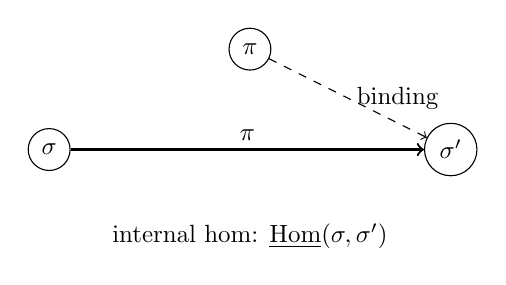
\begin{tikzpicture}[scale=0.85, every node/.style={scale=0.9}]
  \node (A) at (0,0) [draw, circle] {$\sigma$};
  \node (B) at (3,1.5) [draw, circle] {$\pi$};
  \node (C) at (6,0) [draw, circle] {$\sigma'$};
  \draw[->, thick] (A) to node[above] {$\pi$} (C);
  \draw[->, dashed] (B) to node[right] {binding} (C);
  \node at (3,-1.3) {internal hom: $\underline{\mathrm{Hom}}(\sigma,\sigma')$};
\end{tikzpicture}
\caption{Internal hom (causal bind) as morphism object.}
\end{figure}

%=====================================================================
\section{Compiler IR Grammar (Appendix E)}
%=====================================================================

\subsection{EBSSC IR (BNF-like)}

\begin{verbatim}
<program> ::= <decl>*

<decl> ::= sphere <id> ":" <typespec> "{" <modality_list> "}"
         | rule <id> ":" <in_type> "->" <out_type> "budget" <float> "{"
             <impl> "}"
         | func <id> "(" <params> ")" "{" <body> "}"

<typespec> ::= "Sphere" "<" <type> ">"
<modality_list> ::= <modality> ("," <modality>)*
<modality> ::= "text" | "proof" | "audio" | "image" | ...

<stmt> ::= <pop_stmt> | <merge_stmt> | <collapse_stmt> | <assign> | <if> | <while>

<pop_stmt> ::= "pop" <sphere_id> "into" <new_id> "with" <rule_id> ";"
<merge_stmt> ::= "merge" <sphere_id> "," <sphere_id> "into" <new_id> ";"
<collapse_stmt> ::= "collapse" <sphere_id> "into" <new_id> ";"

<expr> ::= <id> | <literal> | <call>
\end{verbatim}

\subsection{IR Type Checking Pass}
The type checker ensures:
\begin{itemize}
    \item rule input types match sphere modalities,
    \item declared budgets sum to $\le B$ on any path,
    \item provenance edges are well-formed hashes.
\end{itemize}

\subsection{IR Lowering}
Lowering maps IR to executable trace:
\[
\text{IR} \xrightarrow{\text{lower}} \text{Trace} = (\sigma_0,\pi_1,\sigma_1,\ldots)
\]
with budget annotations and solver hints.

%===================================================================== \section{Symbol Index and Notation (Appendix F)} %===================================================================== \begin{longtable}{p{2.6cm} p{11cm}} \toprule Symbol & Meaning \\ \midrule $\sigma$ & Semantic sphere (region + internal field + metadata) \\ $\Phi$ & Internal semantic field (vector/scalar) \\ $\partial\Phi$ & Boundary field / interface \\ $E(\sigma)$ & Semantic entropy of sphere \\ $\pi$ & Policy operator (latent action) \\ $\Lambda$ & Sparsity pressure (L1 coefficient) \\ $C(\pi)$ & Cost of policy $\pi$ (compute/metabolic) \\ $G(\sigma,\pi)$ & Expected free energy functional \\ $\oplus,\circledast,\ominus$ & pop (expand), merge, collapse operators \\ $\mathcal{P}$ & Latent policy space \\ $\mathcal{F}$ & Free-energy functor mapping morphisms to $\R_{\ge0}$ \\ $\lambda_c$ & Critical entropy coupling threshold \\ $B$ & Global entropy budget \\ $\Delta E(\pi)$ & Entropy increment of applying $\pi$ \\ $\|\cdot\|_1,\|\cdot\|_0$ & L1 norm (sparsity) and L0 pseudo-norm \\ $U$ & Unitary lift matrix (for unistochastic mapping) \\ $B_{ij}$ & Unistochastic matrix $B_{ij}=|U_{ij}|^2$ \\ $\mathcal{R}$ & Entropy-coupled inference functional $\Phi - \lambda\Sigma$ \\ \bottomrule \end{longtable} %===================================================================== % Bibliography %===================================================================== 

\bibliographystyle{plain}
\bibliography{ebssc_refs}
\end{document} 